\documentclass[a4paper,10pt,twoside]{cpc-hepnp}

\usepackage{multicol}
\usepackage{xcolor}
\usepackage{graphicx}
\usepackage{booktabs}
\usepackage{amssymb,bm,mathrsfs,amscd}
\usepackage[tbtags]{amsmath}
\usepackage{lastpage}
\usepackage{CJK}
\usepackage{subfigure}
\usepackage{booktabs}  %  ???????
\usepackage{amsfonts}
\usepackage{subfigure}
\usepackage{float} 
\usepackage{siunitx}
\usepackage{ulem}

\begin{document}
%\begin{CJK*}{GBK}{song}
\begin{CJK*}{GB}{gbsn}

  \fancyhead[c]{\small PREPARED FOR SUBMISSION TO CPC}
  \fancyfoot[C]{\small 010201-\thepage}

\footnotetext[0]{}

\title{Calibration Strategy of the JUNO Experiment}

\author{%
      %Author1$^{1,2;1)}$\email{someone@sjtu.edu.cn}%
\quad JUNO collaboration$^{1)}$\email{xxx}%
}
\maketitle


\address{%
  $^1$ School of Physics and Astronomy, Shanghai Jiao Tong University, Shanghai Key Laboratory for Particle Physics and Cosmology, Shanghai, 200240, China  \\
%$^2$ {\bf Example}: Institute of High Energy Physics, Chinese Academy of Sciences, Beijing 100049, China\\
}


\begin{abstract}
  We present the calibration strategy for the 20 kton liquid
  scintillator central detector of the Jiangmen Underground Neutrino
  Observatory. By utilizing a comprehensive multiple-source,
  multiple-position calibration program, in combination with a dual
  calorimetry approach with two independent sets of photosensors, we
  demonstrate that the JUNO central detector can achieve a better than
  1\% linear energy scale and a superior 
  effective energy resolution of 3\%,
  required by the neutrino mass hierarchy determination.
\end{abstract}

\begin{keyword}
  JUNO, Neutrino mass hierarchy, Calibration, Radioactive sources,
  Double calorimetry
\end{keyword}

\begin{multicols}{2}

\section{Introduction}
%\subsection{Importance of calibration}
The massive nature of neutrinos have been firmly established by the
neutrino oscillation experiments~\cite{PDG,McKeown-and-Vogel}, but the
ordering of the three mass eigenstates, $m_1$, $m_2$, and $m_3$,
remains unclear. The solar neutrino experiment has established that
$m_2 > m_1$. The gap between $m_3$ and ($m_1$,$m_2$) is significantly larger,
but experimentally there has been no clear evidence
whether $m_3$ is the largest or smallest. This is the so-called
neutrino mass hierarchy (MH) problem.

The Jiangmen Underground Neutrino Observatory (JUNO) is a
multi-purpose experiment to elucidate fundamental neutrino properties
as well as to study neutrinos with astrophysical or terrestrial
origins~\cite{yellow-book}. Its central detector (CD) is a 20-kton
liquid scintillator (LS) detector, located 700~m underground in
Guangdong, China. The detector is at an equal distance of 53 km from
the Yangjiang and Taishan nuclear power plants along the south China
coast. Such a median baseline configuration is ideal for the
determination of neutrino MH using the electron anti-neutrinos from
the reactors~\cite{petcov-original-paper, petcov2, learned,
  zhanliang-original-paper-2008}. Due to neutrino oscillation, the
survival probability of anti-electron neutrinos can be written as:
\begin{eqnarray}
\label{eq_p_neutrino}
\begin{aligned}
  &P_{\overline{\nu_{e}} \rightarrow \overline{\nu_{e}}} = 1-\sin ^{2}2\theta_{13}\times\\
  &\left( \cos^{2}\theta_{12} \sin^{2}(\Delta m_{31}^2\frac{L}{4E^{\nu}}) +\sin ^{2} \theta_{12} \sin ^{2}(\Delta m_{32}^2\frac{L}{4E^{\nu}}) \right) \\
  & -\cos ^{4} \theta_{13} \sin ^{2} 2 \theta_{12} \sin ^{2}(\Delta
  m_{21}^2\frac{L}{4E^{\nu}})
\end{aligned}
\end{eqnarray}
In this expression, $\theta_{12}$ and $\theta_{13}$ are the neutrino
mixing angles, $\Delta m_{ij}^2 \equiv m_i^2 - m_j^2$ is the
mass-square-difference between eigenstates $i$ and $j$, $L$ is the
distance from neutrino production to detection (baseline), and
$E^{\nu}$ is the energy of the neutrino. Numerically, $|\Delta
m_{32}^2|$ and $|\Delta m_{31}^2|$ are mostly degenerate
($\sim2.5\times10^{-3}$~eV$^2$), and $\Delta m_{21}^2$ is much less
with a value $\sim7.5\times10^{-5}$~eV$^2$. For the so-called normal
or inverted hierarchy, $|\Delta m_{31}^2| = |\Delta m_{32}^2| \pm
\Delta m_{21}^2$. Due to the fact that $\theta_{12} \sim \ang{30}$,
the two oscillation frequencies driven by $\Delta m_{31}^2$ and
$\Delta m_{32}^2$ are weighted differently in
Eqn.~\ref{eq_p_neutrino} 
and the main information of mass hierarchy come from a region 
with neutrino energy between 3 and 6 MeV
, which allows one to determine the hierarchy
if the oscillation pattern in $E_{\nu}$ can be measured with
unprecedented high precision.

The JUNO LS is contained inside a 35-m diameter acrylic sphere with
12~cm thickness, strengthened by 591 stainless steel (SS) connection
bars. About 18,000 20-inch and 25,000 3-inch photomultipliers (PMTs)
are closely packed and immersed in ultra-pure water outside the sphere
viewing the LS. 
%Modification RED (previous text) and BLUE (new text)
  These two sets of photosensors and their
  corresponding readout electronics, constitute the LPMT (large) and
  the SPMT (small) systems.  The SPMT was introduced to enable a
  redundant calorimetry metric called ``dual calorimetry''.  This
  technique, implemented in JUNO for the first time, exploits the
  complementary differences between of both readout systems to yield
  unique response insight. The electron anti-neutrinos are detected
via the so-called inverse $\beta$-decay (IBD), $\bar{\nu}_{e}+p
\rightarrow e^{+}+n$, where the electron anti-neutrinos interact with
protons in the LS then produce positrons and neutrons.  The positron
will deposit its kinetic energy promptly with a range between 0 to 8
MeV in the LS, then annihilate with an electron producing gamma rays.
The energy of the anti-neutrino is related to the kinetic energy of
the positron as E$^{\nu}$ $\approx$ E$^{e+}+1.8$~MeV. The neutron will
be captured on a proton within about 200~$\mu$s,
producing a delayed 2.22~MeV gamma.

Particle interactions in the LS will produce scintillating
(dominating) and Cerenkov (sub-dominant) photons, which will be
converted to photoelectrons (PE) by the PMTs and read out
by electronics. Let us now consider the nonlinearity of the energy
scale intrinsic to the LS. The scintillation photons has a known
Birks' ``quenching'' effect~\cite{PDG}, and the Cerenkov emission
depends on the velocity of the charged particle. The combined effect
is clearly both energy and particle dependent, and will be referred to
as the ``physics nonlinearity'' hereafter. The PMT instrumentation and
electronics may carry additional ``instrumental nonlinearity'', which
is a nonlinear response between the created photons in the LS and the
measured charge from the electronics. This nonlinearity is
particularly non-trivial for the LPMTs.  
  For a constant energy deposition, the LPMT charge response varies by
  up to 2 orders of magnitude depending on the position due to solid
  angle variations and optics.  For example, a positron with 8~MeV
  kinetic energy produces up to 100\,PE in the closest PMT, and on
  average 0.25\,PE in the farthest one. In this context, the impact of
  instrumental nonlinearity is particularly delicate.  Instead,
  the SPMT was designed to operate mainly in the single photon
  detection in the IBD energy range anywhere in the volume, so charge
  can be estimated either directly or via digital photon counting.
  Since both LPMT and SPMT are exposed to the common energy
  deposition, the SPMT acts as an independent digital and linear
  in-detector reference to the LPMT main system; i.e. enabling the
  dual calorimetry.

In addition to the energy nonlinearity, the photon collection in JUNO
is strongly position dependent due to PMT solid angles, optical
attenuations, reflections at material interfaces, shadowing due to
opaque materials (e.g. SS connection bars), etc.  
  The uncorrected instrumental nonlinearity can mimic an additional
  position non-uniformity, manifested most acutely closer to the
  detector edge where the LPMT charge response vary widely. The dual
  calorimetry based correction allows channel-wise nonlinearity
  control to reduce or disentangle such systematic response
  ambiguities. The residual position non-uniformity, now intrinsic
due to the detector optics and mostly energy independent, has to be
corrected as well to optimize the energy resolution.

The determination of MH imposes that the uncertainty of the positron
kinetic energy scale should be better than 1\%, and the effective
energy resolution should be better than 3\%
~\cite{zhanliang-original-paper-2009,zhanliang-original-paper-2013,yellow-book}.
These stringent requirements can only be achieved through a
comprehensive calibration program. In this paper, we describe the
calibration strategy for JUNO and demonstrate how the physics needs are satisfied. 
The remainder of the paper is organized as follows. In
{Sec.~\ref{sec:scale_calib}}, we discuss the approach of the energy
scale calibration to combat the physics and instrumental
nonlinearity. 
We then develop the method to minimize the energy
resolution via correcting the position non-uniformity,
in {Sec.~\ref{sec:resolution}}.  Based on these, we present the
conceptual design of the calibration hardware in
{Sec.~\ref{sec:CalibSys}}, and the calibration program that we
envision in {Sec.~\ref{sec:calib_program}}, before concluding in
{Sec.~\ref{sec:summary}}.

\section{Energy scale calibration}
\label{sec:scale_calib}
A custom Geant4-based (version 9.4.p04)~\cite{Geant4} software, called
SNIPER~\cite{SNIPER}, is used to perform calibration related
simulations. SNIPER consists of the up-to-date JUNO detector
geometries and optical parameters. The JUNO LS was
  tested in an decommissioned Daya Bay detector, so the LS optical
  parameters such as the light yield, absorption and re-emission
  probability were tuned to the data~\cite{YuZeyuan_LSpaper,
    JUNOLSAbsL}. The Rayleigh scattering length was measured in a
  separate bench experiment~\cite{Zhouxiang_Paper}. The optical parameters of the
  acrylic sphere, ultrapure water, and other materials were taken from
  bench measurements. The quantum efficiency and collection efficiency
  (angle-dependent) of the LPMT and SPMT were initially set at the
  average values from quality assurance tests, and can be adjusted
  individually in the simulation. The so-called ``low energy'' physics
  lists for the electron, positron and gamma are selected in SNIPER,
  based on the Daya Bay experience.

\begin{center}
  	%\tabcaption{Radioactive sources} \footnotesize
  \tabcaption{List of radionuclides considered in the JUNO calibration
    system. For the $^{68}$Ge source, it decays into $^{68}$Ga via
    electron capture, then $\beta^{+}$-decay into $^{68}$Zn.  Although
    being a positron emitter, the kinetic energy of the positron will
    be absorbed by the enclosure, so only the annihilation gammas will
    be released.}
	\label{radioactive_source}
	%\begin{tabular}{c@{\extracolsep{\fill}}|c|c|ccc}
        %\toprule  % ???
	%\begin{tabular}{@{\extracolsep{\fill}}c|c|c}\hline
        \begin{tabular}{c|c|c}\hline 
          Source & Type & Radiation\\\hline 
          %\midrule  % ???
          $^{137}$Cs& $\gamma$ & 0.662 MeV\\
          $^{54}$Mn & $\gamma$ & 0.835 MeV\\
          $^{60}$Co & $\gamma$ & 1.173 + 1.333 MeV\\
          $^{40}$K  & $\gamma$ & 1.461 MeV\\
          %\midrule  % ???
          $^{68}$Ge & e$^{+}$ & annil 0.511 + 0.511 MeV\\
          %\midrule
          $^{241}$Am-Be & n, $\gamma$ & neutron + 4.43 MeV \\
          $^{241}$Am-$^{13}$C &n, $\gamma$ & neutron + 6.13 MeV \\
          (n,$\gamma$)p & $\gamma$ & 2.22 MeV \\
          (n,$\gamma$)$^{12}$C & $\gamma$ & 4.94 MeV or 3.68 + 1.26 MeV\\\hline
          %\bottomrule  % ???
	\end{tabular}

\end{center}

\subsection{Calibration of physics nonlinearity}
\subsubsection{Selection of sources}
For a large LS detector, thin-walled electron or positron sources
would pose risk on leakage of radionuclides and difficulties on
blockage of photons due to non-transparent materials (referred to as the shadowing effect hereafter). 
For simplicity, we consider $\gamma$ sources
ranging from a few hundred keV to a few MeV to cover the range of the
prompt energy the IBDs. In addition, ($\alpha$,n) sources
$^{241}$Am-Be (AmBe) and $^{241}$Am-$^{13}$C (AmC) can be used to both
provide high energy gammas, as well as neutron capture signals on
proton and carbon. The sources and types of radiations are listed in
Table~\ref{radioactive_source}.

\subsubsection{Model of physics nonlinearity}
\label{sec:nonlin}
Most IBD positrons lose energy by depositing ionization energy (the
same way as electrons) before they stop. A positron can either
directly annihilate with an electron, or form either a para- or
ortho-positronium bound state before it
annihilates~\cite{borexino-positronium-paper}, producing either two or three
gammas, respectively, with a total energy of 1.022 MeV. Therefore, the
observed prompt energy of an IBD can be written as
\begin{eqnarray}
\label{E_eplus_vis}
E_{\rm prompt} = E_{\rm vis}^{e} + E_{\rm vis}^{\rm anni}\,.
\end{eqnarray}


The first term describes the visible energy associated with the
kinetic energy of the positron, which would be identical for an
electron with the same energy, and the second term is the visible
energy of the annihilation gammas.  $E_{\rm vis}^{\rm anni}$ can be
approximately calibrated using an enclosed $^{68}$Ge source, although
the IBD positron has sub-percent of probability of annihilating in
flight, emitting higher energy gammas. Let us now define a physics
nonlinearity
\begin{equation}
\label{E_nonlin}
f_{\rm nonlin} = \frac{E_{\rm vis}^e}{E^e}\,,
\end{equation}
in which $E^e$ is the true kinetic energy of an electron or
positron. So if $f_{\rm nonlin}$ can be determined via calibration,
then for each IBD event, the true kinetic energy of a positron can be
reconstructed as
\begin{equation}
\label{eq:positron_energy_rec}
E^{e} = \displaystyle\frac{E_{\rm prompt}-E_{\rm vis}^{\rm anni}}{f_{\rm nonlin}}\,.
\end{equation}


A gamma converts its energy into the LS via secondary electrons. This
internal connection allows a robust determination of $f_{\rm nonlin}$
using the gamma calibration
data~\cite{kamland-calibration-paper,dayabay-first-shape-paper}. Without
loss of generality, let us model $f_{\rm nonlin}$ as a four parameter
function, as used in the first Daya Bay spectral
analysis~\cite{dayabay-first-shape-paper},
\begin{eqnarray}
\label{Ele_nonlin}
f_{\rm nonlin} = \frac{p_{0}+p_{3}E^e}{1+p_{1}e^{-p_{2}E^e}}\,, 
\end{eqnarray}
where the exponential on the denominator enforces a decay of the
physical nonlinearity at higher energy.


Let $P(E^{e})$ denote the probability density function (PDF) of a
given gamma source converting to secondary electrons/positrons via the
Compton scattering, photoelectric effect, or pair production, at an
energy $E^{e}$, determined from the simulation model. Then the visible
energy of the gamma is simply

\begin{equation}
\label{eq_gamma}
E_{\rm vis}^{\gamma} = \int P(E^e)\times f_{\rm nonlin}(E^e) \times E^{e} dE^e\,.
\end{equation}
Multiple sources in Table~\ref{radioactive_source} lead to multiple
Eqn.~\ref{eq_gamma}, so parameters in Eqn.~\ref{Ele_nonlin} can be
determined with redundancy.

  The highest gamma energy point is 6.13~MeV (AmC),
  which is insufficient to cover the full energy range of IBD
  positrons. On the other hand, cosmogenic $\beta$ background such as
  $^{12}$B ($Q$ value 13.4~MeV) is abundant in JUNO, about 1000 evts
  per day~\cite{yellow-book}. $^{12}$B decays with a half life of
  20~ms, which can be clearly identified by looking for delayed high
  energy $\beta$ event (with a few percent mixture of $^{12}$N, a
  $\beta^{+}$-emitter) after an energetic
  muon~\cite{kamland-cosmogenic-bkg-paper}.  More than 98\% of the
  $^{12}$B $\beta$-decay into the ground state of $^{12}$C, making it
  almost a pure $\beta$ source. Therefore, despite its continuous
  spectrum, $^{12}$B offers complementary constraints to
  $f_{\rm nonlin}(E^e)$ at the high energy end.  To combine the gamma
  source and $^{12}$B data, we define a $\chi^{2}$ as
\begin{equation}
\label{eq_chi2}
%\chi^{2}=\chi_{\gamma}^{2}+\chi_{B 12}^{2}=\sum_{j}^{8}\left(\frac{M_{j}^{\gamma}-P_{j}^{\gamma}}{\sigma_{j}}\right)^{2}+\sum_{i=0}^{100} \frac{\left(M_{i}^{B 12}-P_{i}^{B 12}\right)^{2}}{M_{i}^{B 12}}
\chi^{2}=\sum_{j}^{8}\left(\frac{M_{j}^{\gamma}-P_{j}^{\gamma}}{\sigma_{j}}\right)^{2}+\sum_{i=0}^{100} \frac{\left(M_{i}^{\rm B12}-P_{i}^{\rm B12}\right)^{2}}{M_{i}^{\rm B12}}
\end{equation}
where $M_{j}^{\gamma}$ and $P_{j}^{\gamma}$ are the measured and
predicted visible energy peak of the $j$th gamma source, respectively,
and $\sigma_{j}$ is the corresponding uncertainty. The $^{12}$B
spectrum will be binned, and $M_{i}^{\rm B12}$ and $P_{i}^{\rm B12}$
are the number of measured and predicted events, normalized to the
total measured events, in the $i$th visible energy bin.

\subsubsection{Validation of calibration procedure}
To validate this procedure, we use SNIPER to simulate bare gamma
sources in Table~\ref{radioactive_source} at the center, and $^{12}$B
decays uniformly distributed in the entire detector. 
The visible energy $E_{\rm vis}$ is estimated from the total PE by assuming a
somewhat arbitrary scaling constant ($\sim$1345 PE/MeV) set by the 2.22
MeV gammas from the neutron-proton captures at the CD center.  For
each gamma source, the corresponding PDF $P(E^e)$ is extracted from
the underlining Geant4 processes. For the$^{12}$B data, a cut of 5 MeV
is applied to remove accidental background due to intrinsic $^{208}$Tl
in the liquid scintillator. In addition, a fiducial cut of a radius of
less than 15~m is chosen to avoid energy leakage via Bremstralung
close to the boundary. The data are also corrected for position
non-uniformity using the procedure in later {Sec.~\ref{sec:non-uni}}. To
obtain the predicted $^{12}$B spectrum, the physics non-linearity
(Eqn.~\ref{Ele_nonlin}) as well as a spectral smearing according to
the energy resolution function (Eqn.~\ref{eq_resolution}) are applied
in each iteration of the fit.  The statistical uncertainty of each
gamma peak is estimated to be better than 0.01\% with 100,000
calibration events. The statistics of $^{12}$B is assumed to be
equivalent to one month running period, with approximately 70\%
fiducial acceptance.

\begin{figure}[H]
  \centering 
  \subfigure[Gamma nonlinearity] {
    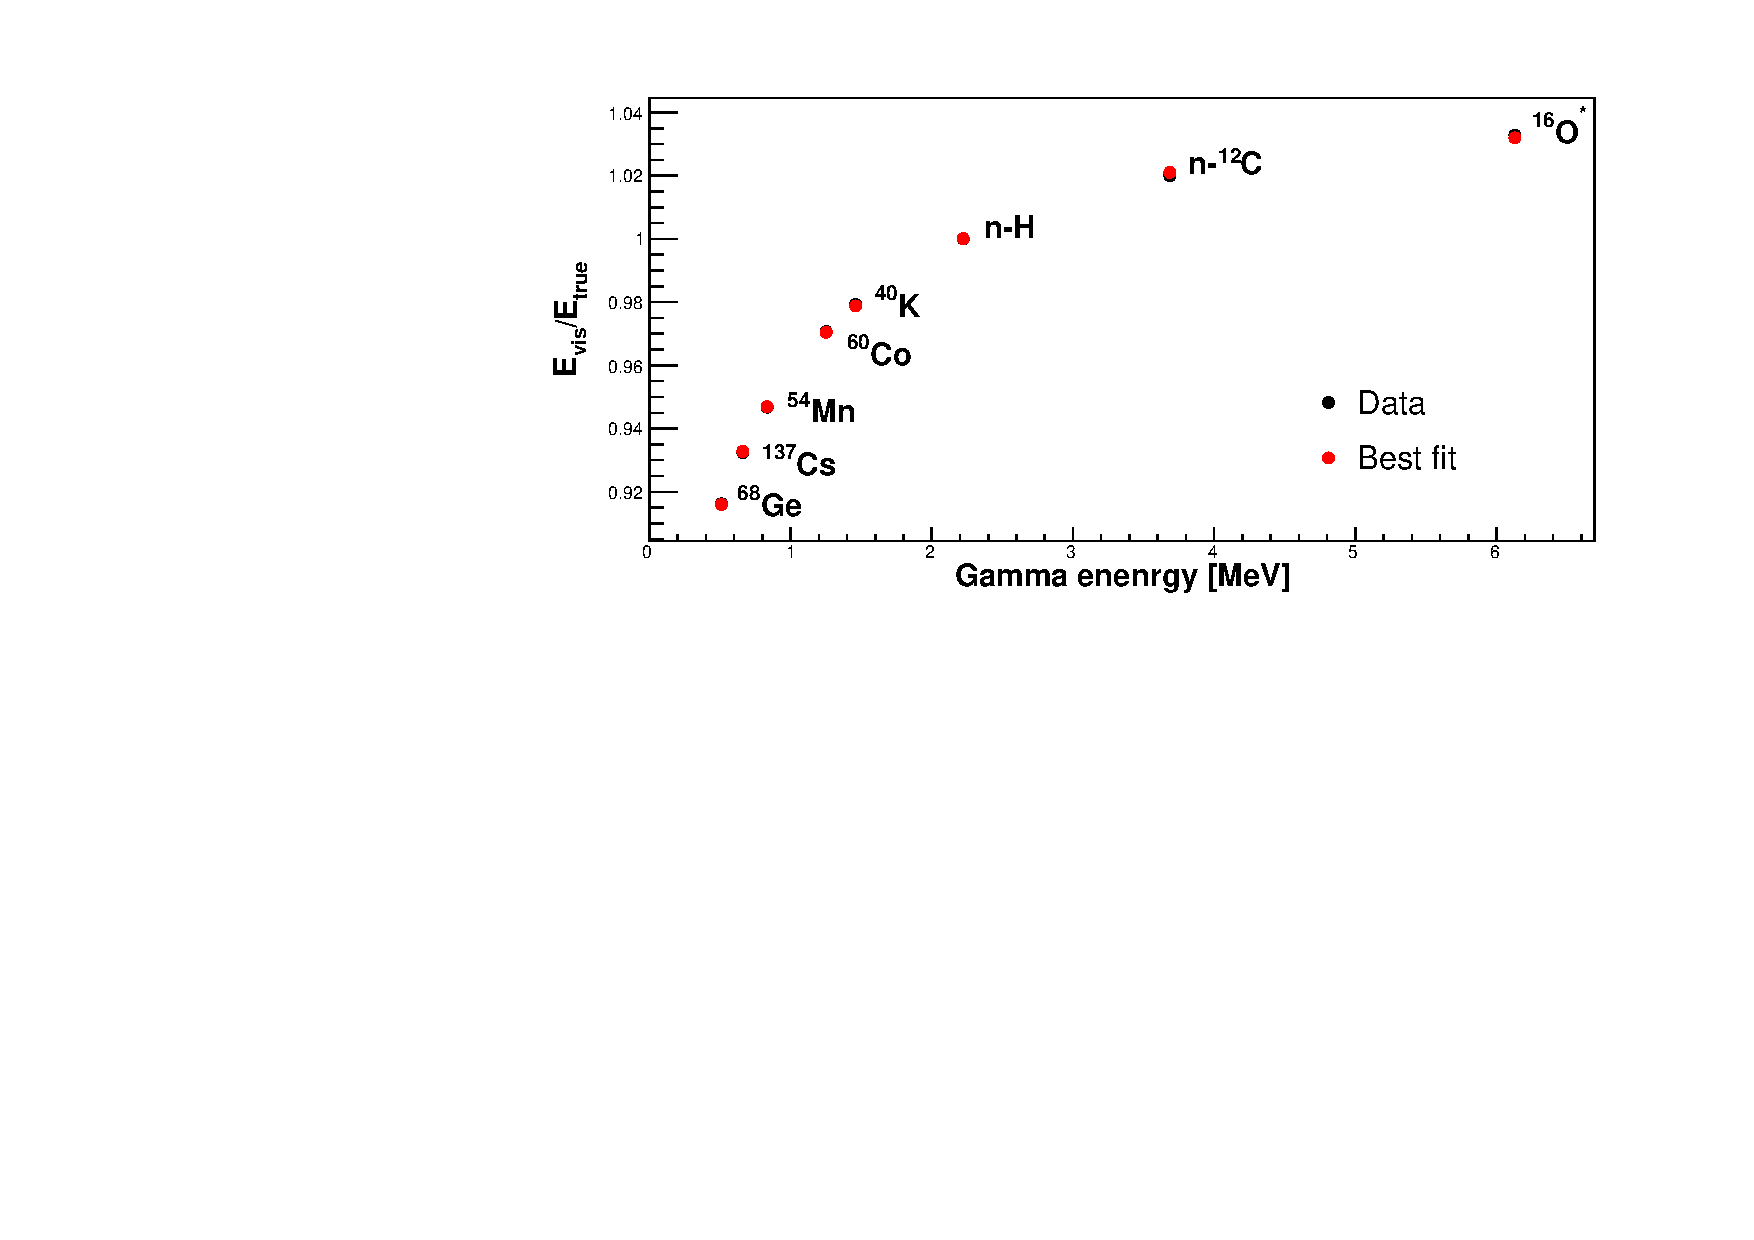
\includegraphics[width=3in]{non_linearity.pdf}
    \label{non_linearity_fit}
  }
  \subfigure[Boron Spectrum] {
    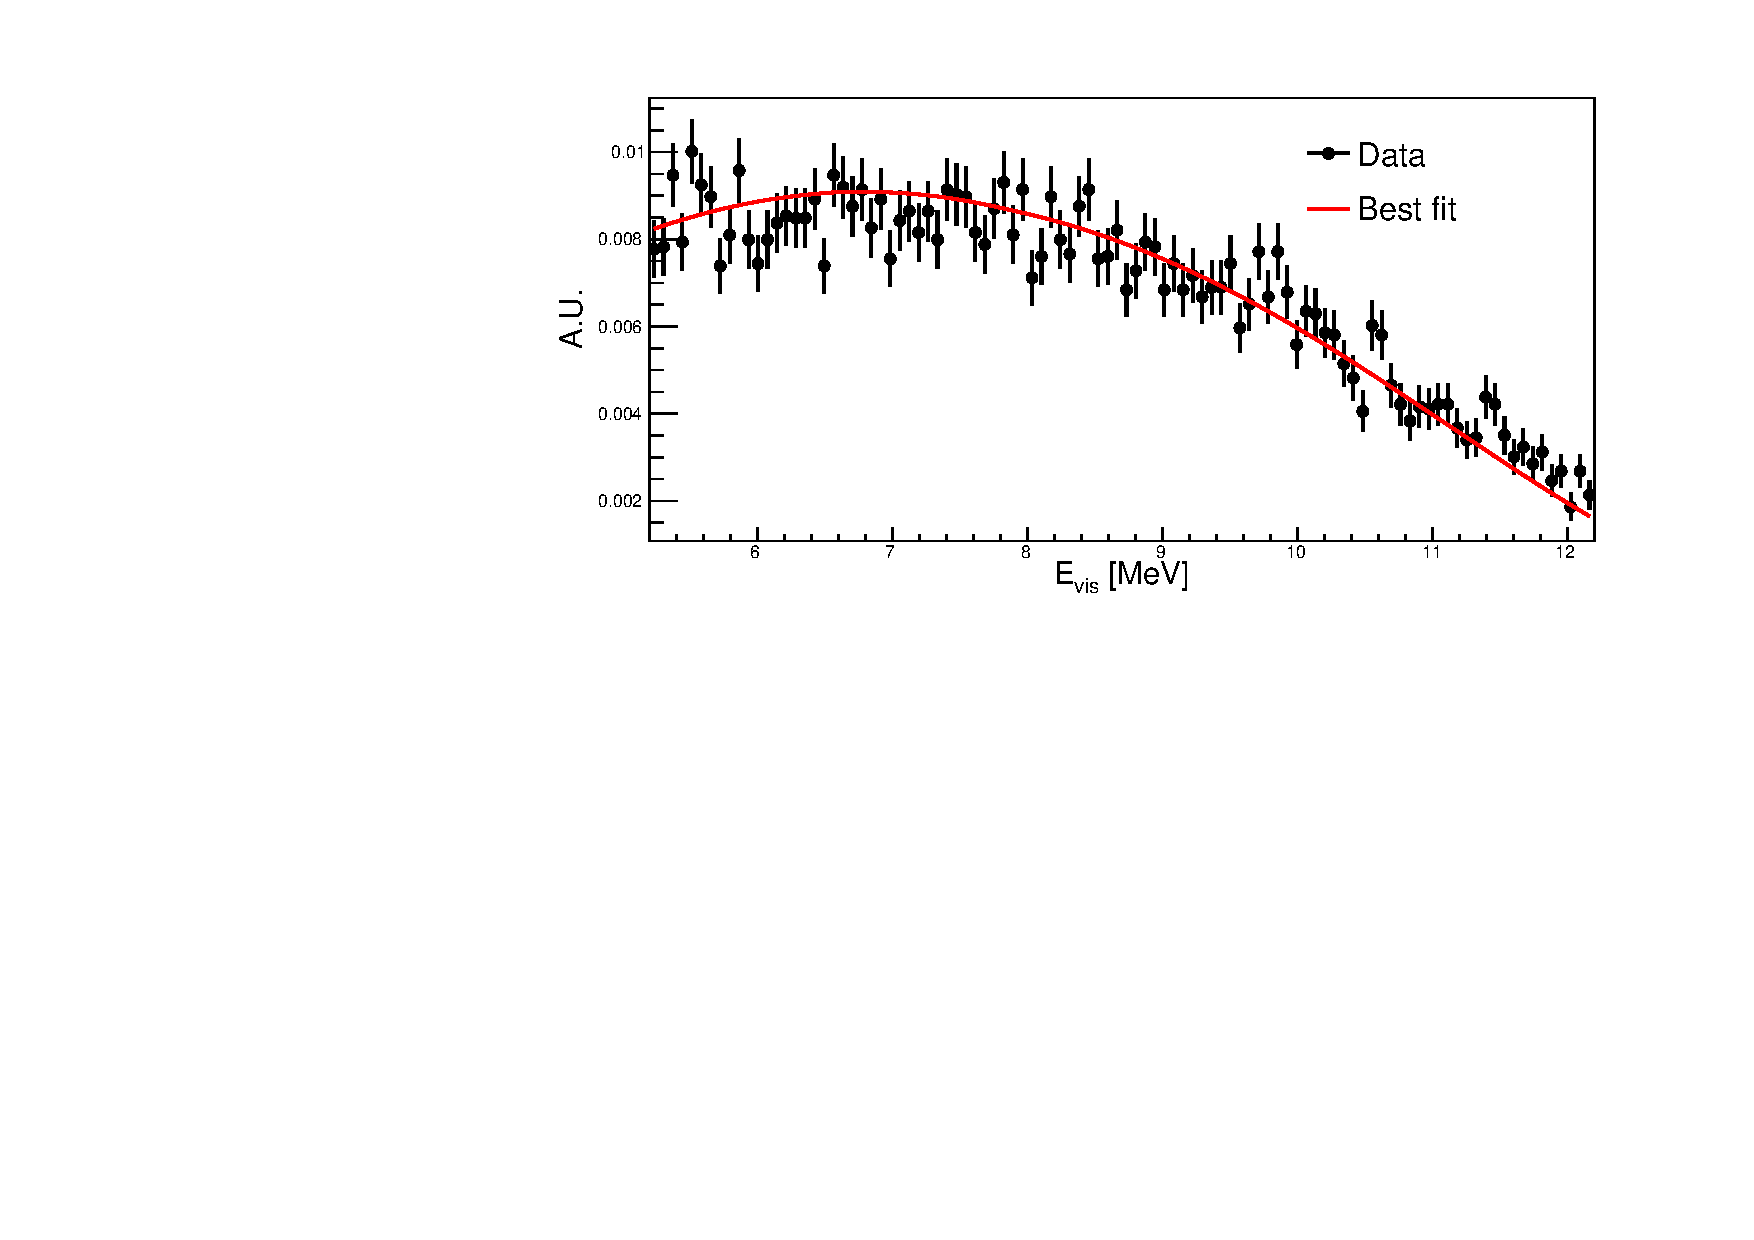
\includegraphics[width=3in]{B12.pdf}
    \label{B12}
  }
  \subfigure[Electron nonlinearity] {
    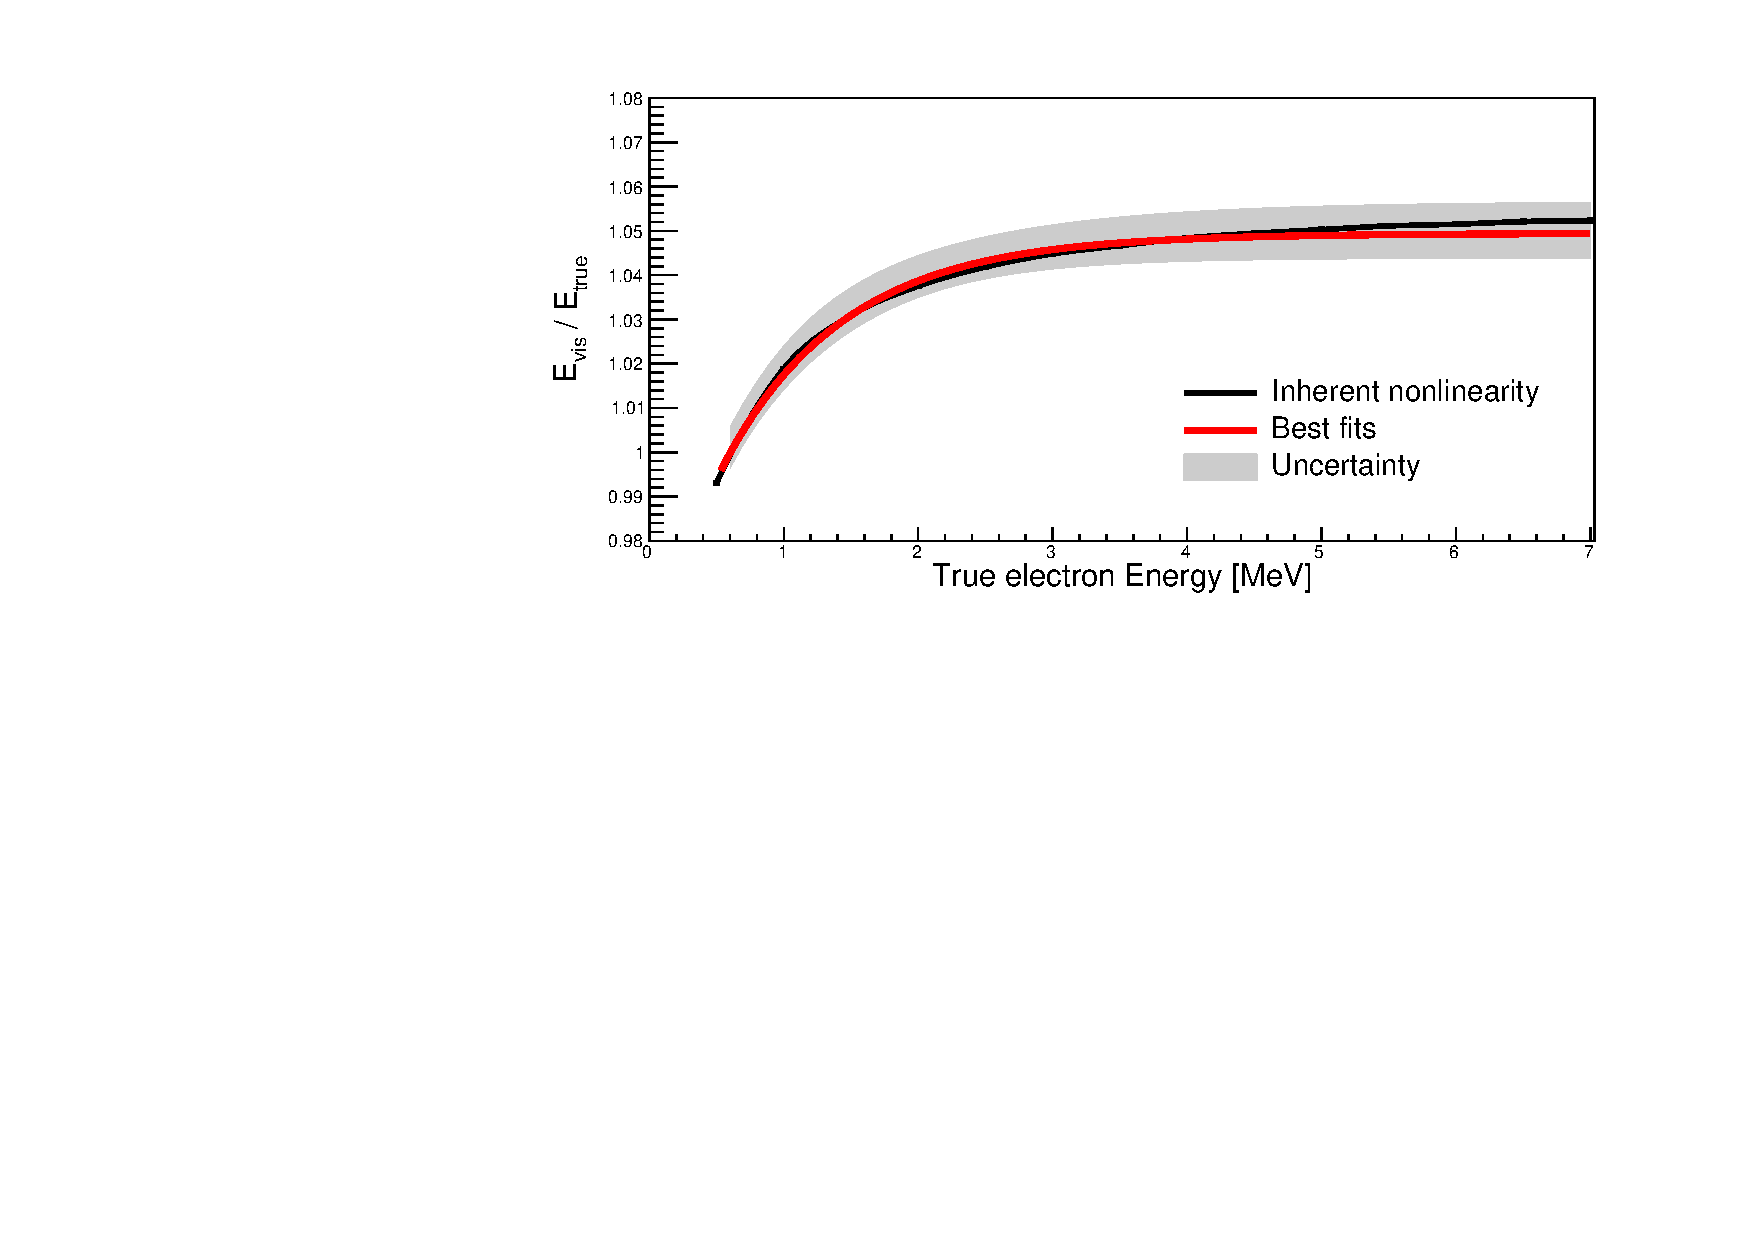
\includegraphics[width=3in]{non_ele_fit_truth.pdf}
    \label{non_e_linearity_fit}
  }
  \caption{Fitted and simulated gamma nonlinearity(a), $^{12}$B
    spectra (b), and electron nonlinearity (c). In all figures, black
    points (curve) represent the simulated data, and the red points
    (curves) are the best fits. Statistical uncertainties for the
    gamma sources are at a 0.01\% level so are invisible from the
    figure. The 4.43 MeV gamma from the Am-Be neutron source is not
    used, as it is contaminated by the simultaneous nuclear recoil
    signals.  In (b), the spectrum corresponds to roughly one month of
    $^{12}$B data in the detector, and smearing due to energy
    resolution is included in the fit. In (c), the uncertainty band is
    evaluated using the procedure in Sec.~\ref{sec:sys}.  }
\end{figure}
With the above input, $p_i$ is determined by Eqn.~\ref{eq_gamma} using
the $\chi^2$ fit (Eqn.~\ref{eq_chi2}). For the gamma sources, the
ratios of the best fit visible energy (Eqn.~\ref{eq_gamma}) to the
true are compared to those from the simulated data in
Fig.~\ref{non_linearity_fit}, where excellent agreement is found. 
For visual clarity, 
for sources with multiple gamma emissions, the
horizontal axis is chosen to be the mean energy of the gammas.  The
best fit model for the $^{12}$B visible spectrum is overlaid with
simulated data in Fig.~\ref{B12}, where good agreement is also
observed.  For comparison, we use the same SNIPER to produce the
visible energy for individual mono-energetic electrons at the CD
center and extract the true $f_{\rm nonlin}$. 
Assuming no charge nonlinearity effects, the difference between
best fit and the true electron nonlinearity is better than a
0.3\% within the entire energy range, as shown in
Fig.~\ref{non_e_linearity_fit}.


For a final sanity check, we perform SNIPER simulation on
mono-energetic positrons at the CD center. The kinetic energy is
reconstructed event-by-event using Eqn.~\ref{eq:positron_energy_rec},
in which $E_{\rm vis}^{\rm anni}$ is obtained from the simulation of
an enclosed $^{68}$Ge source and $f_{\rm nonlin}$ is taken from the
best gamma fit in the previous step. The residual bias in the
reconstructed energy and the 1$\sigma$ uncertainty band (see
Sec.~\ref{sec:sys}), as depicted in
Fig.~\ref{fig:positron_nonlinearity}, is less than 0.6\% over the
entire range of the IBD energy, which is significantly better than the
1\% requirement.

\begin{center}
  \centering
  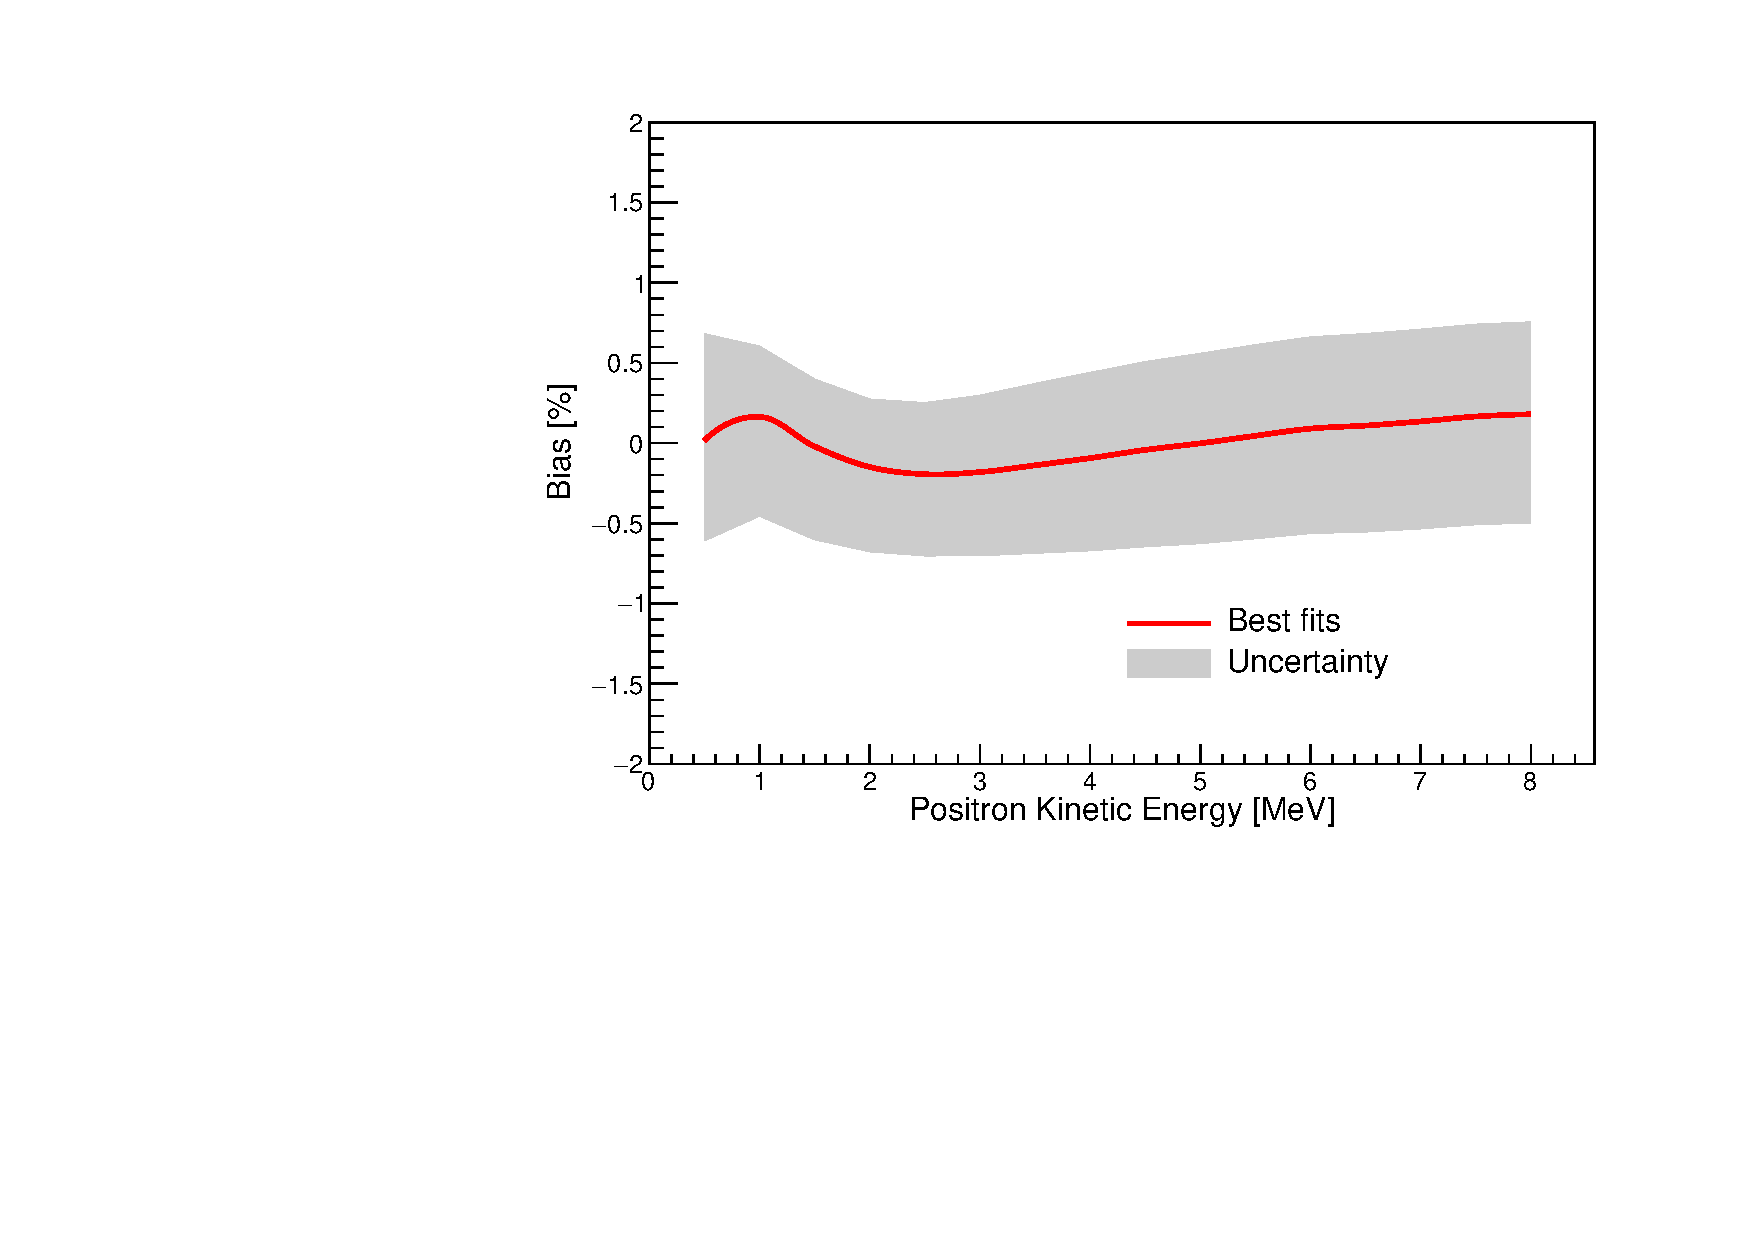
\includegraphics[width=3in]{non_eplus_bias.pdf}
  \figcaption{Bias in the reconstructed positron kinetic energy as a
    function of true energy in the SNIPER simulation. The band
    represents the uncertainties in the calibration procedure,
    detailed in Sec.~\ref{sec:sys}. The lowest kinetic energy in the
    figure is 0.5~MeV, to avoid artificial increase of the fractional
    bias when the kinetic energy approaches zero. The best
    fit does not center in the uncertainty band, as some systematic
    uncertainties are one-directional, e.g. the shadowing effect and energy
    loss effects.  }
  \label{fig:positron_nonlinearity}
\end{center}

\subsection{Calibration of instrumental nonlinearity}
\label{sec:elec_nonlin}
  The event-wise instrumental nonlinearity reflects the
  convolution of the channel-by-channel nonlinearity
  contributions. The nonlinearity fraction of each channel depends on
  the illumination, which depends on the location of the energy
  deposition. The best way to correct this is to calibrate each
  channel nonlinearity using a tuneable light source over the full
  illumination dynamic range: from a fraction of a PE up to around
  100\,PE per channel on average. To achieve a uniform illumination in
  all LPMTs with a linear intensity reference (SPMT), one should
  deployed the light source at the center of the CD with an intensity
  varying from 0.3\,MeV (threshold) up to 1.0\,GeV equivalent.
Such a system is demonstrated in Ref.~\cite{zhangyuanyuanpaper},
consisting of a ns-timing pulsed UV laser beam, directed into an
optical fiber with a diffuser ball attached to its open end deployable
along the central axis of the CD. The UV photon at 266 nm is foreseen
to excite the LS thus enabling an output photon time profile similar
to physics events.  The combination of the dual calorimetry design and
the deployable laser source is particularly powerful.
%Modification RED (previous text) and BLUE (new text)
  The SPMT response is made linear in charge by design,
  therefore the total SPMT charge is an ideal in-detector light
  intensity reference, allowing a clean extraction of the LPMT
  channel-wise nonlinearity with varying laser intensity.
  This dual calorimetry metric cancels common effects between the LPMT
  and SPMT.
  Such a calibration scheme can yield remarkable performance, as
  illustrated in Fig.~\ref{fig:inst_nonlinearity}. Electron events
  from 1 to 8~MeV are uniformly simulated in the JUNO CD. We start
  with a very pessimistic LPMT response non-linearity (i.e. a
  channel-wise bias of 50\% over 100\,PE), which induces a seemingly
  energy dependent non-uniformity. For instance, if the non-uniformity
  obtained with 1~MeV energy deposition ({Sec.~\ref{sec:resolution}})
  is applied to correct the event-wise total charge of LPMT for all
  events, the mean bias in energy measurement in the fiducial volumn
  can still be as large as 2\% at 8 MeV. For comparision, if the LPMT
  charge is calibrated channel-wise using the laser and SPMT, the
  event-wise residual instrumental nonlinearity is reduced to
  $\leq$0.3\%. Under more reasonable LPMT nonlinearity assumptions,
  the dual calorimetry laser calibration is expected to yield an
  event-wise linear instrumental response of better than 0.1\%.

\begin{center}
  \centering
  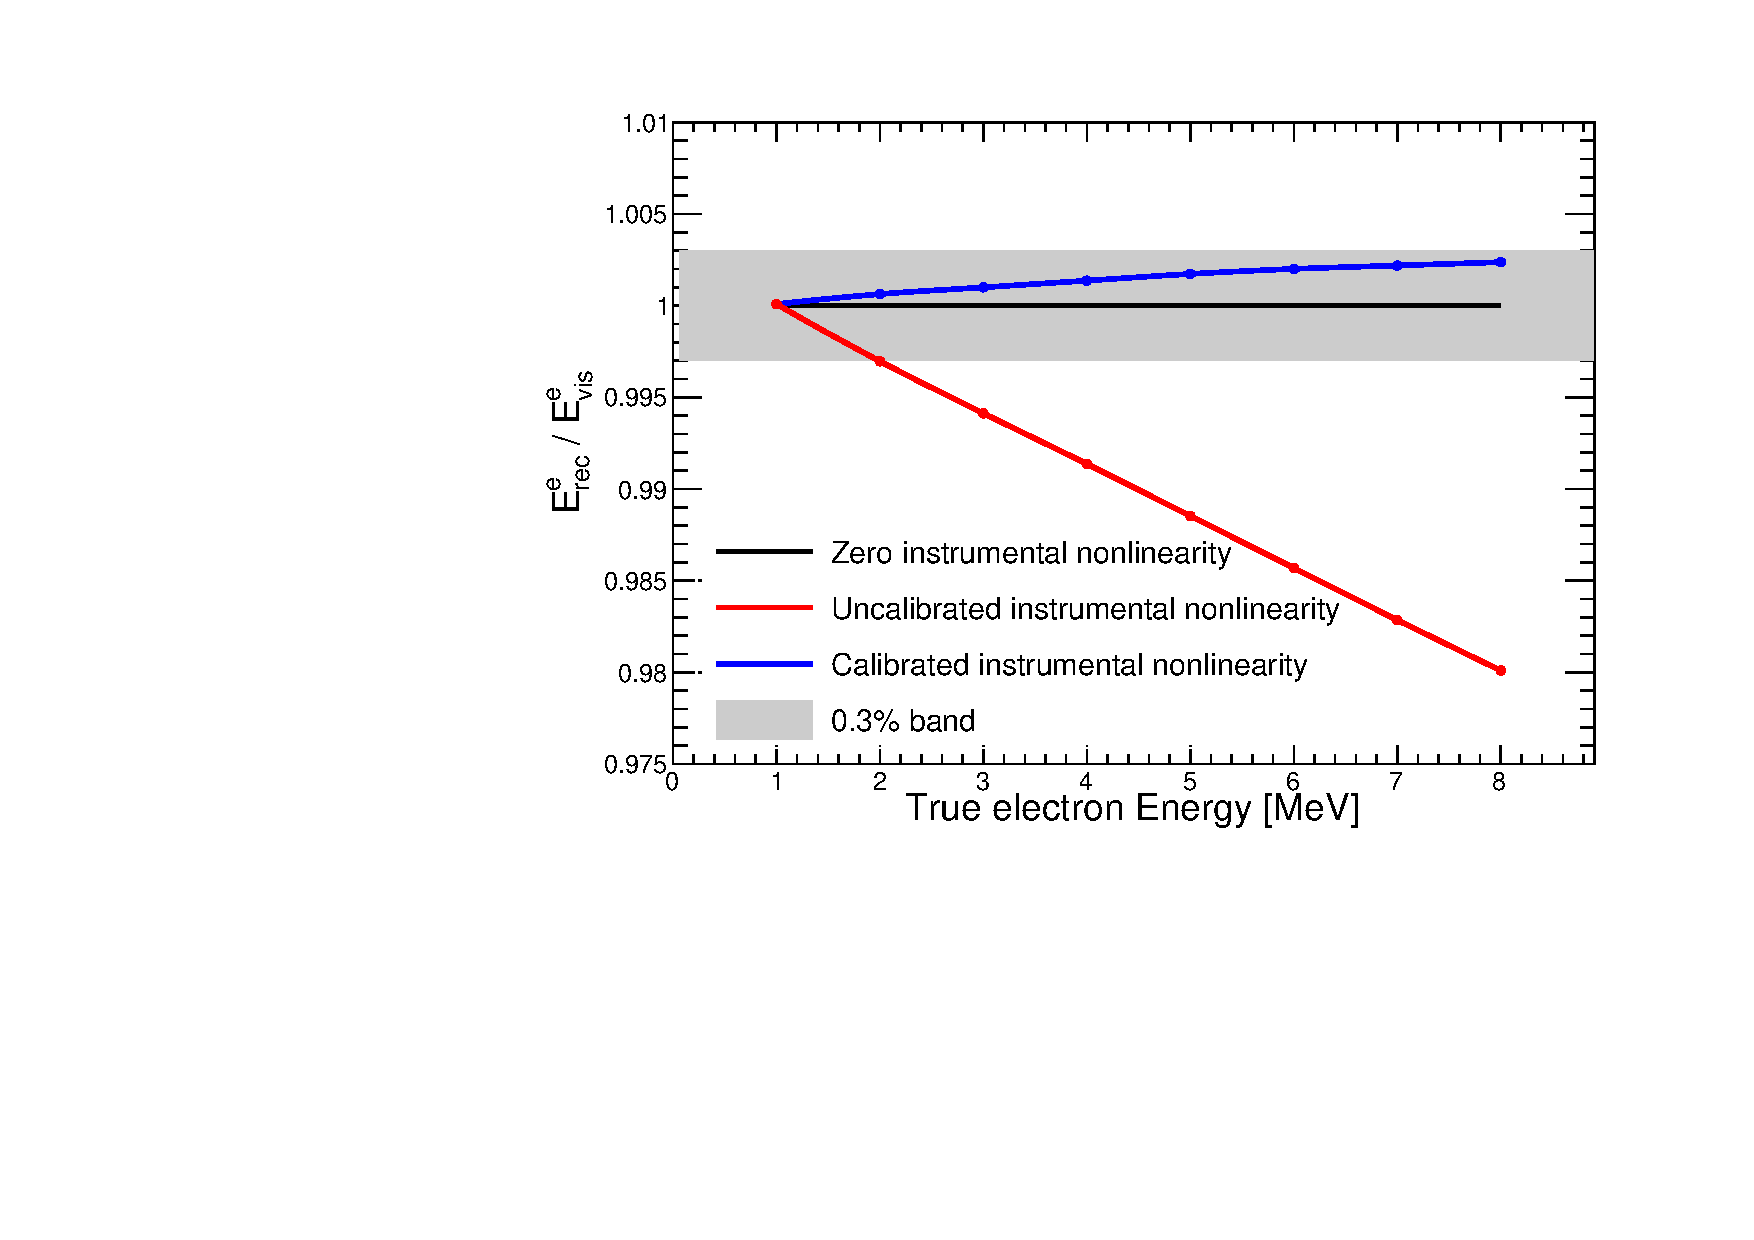
\includegraphics[width=3in]{Plot_instrumental_nonlinearity_calibration.pdf}
  \figcaption{Illustration of the impact of a large instrumental
  nonlinearity to the average energy scale of electrons (uniformly
  distributed in the detector) with and without channel-wise
  correction. 
  The vertical axis is the ratio of the
  reconstructed energy based on measured charge from LPMT to the
  visible energy based on true charge of LPMT.
  The black line
  represents the perfect linear case. For the channel-wise
  instrumental nonlinearity for the LPMT, we assume that it grows
  linearly with the true charge, reaching 50\% at 100\,PE. Its impact
  to the full volume event-wise energy scale, corrected for the
  position non-uniformity at 1 MeV, is shown as the red line. The same
  event-wise energy scale, corrected for the channel-wise nonlinearity
  using the laser and dual calorimetry approach, is shown as the blue
  line.The grey band illustrates the residual uncertainty (0.3\%) of
  this correction.}
  \label{fig:inst_nonlinearity}
\end{center}


%Modification RED (previous text) and BLUE (new text)
	Any laser based nonlinearity calibration could suffer
  from residual biases arising from the time profile of optical
  photons, if the instrumental nonlinearity depends on the photon
  arrival time profile. The excitation time profile of laser may not
  be identical to that from the physical events, and even identical,
  the timing smearing due to for example Rayleigh scatterings is
  vertex dependent, not reflected by the center-only laser
  calibration.  Such an effect can be well controlled by deploying a
  radioactive source and the UV laser to a same series of off-center
  positions.

Since the SPMT system is always monitoring the response of the
detector with or without calibration sources, aside from the
instrumental linearity, the SPMT offers unique insights on the
detector uniformity and the stability of the LPMT response across the
life-span of the experiment.

\subsection{Evaluation of systematic uncertainties}
\label{sec:sys}
The calibration methodology discussed above inevitably bares
systematic uncertainties. We study these uncertainties, and evaluate
the combined effects to the positron energy scale in this section.

\subsubsection{Shadowing effect}
A realistic source is not a point source. A typical source we
envision in the calibration is shown in
Fig.~\ref{source_weight_QC}. The source is enclosed in a 6~mm by 6~mm
cylindrical SS shell, covered by highly reflective
Polytetrafluoroethylene (PTFE), and attached to a SS wire with 1~mm
diameter.
%To maintain the tension in the wire, two 100~g SS weights
A PTFE connector about 20~cm above the source allows easy exchange of
the source when desired. To maintain the tension in the wire, a weight
covered with PTFE is also attached to the wire below the source, with
a separation of about 20~cm. Despite the PTFE materials, optical
photons can still be absorbed by these surfaces, leading to a small
bias in visible energy.


To study this bias, a conservatively a 90\% reflectivity is assumed
for the PTFE surfaces. Only events with energy fully absorbed in the
LS region are chosen from the simulation to decouple this effect with
the energy loss in dead material (see next). 

\begin{center}
  \centering
  %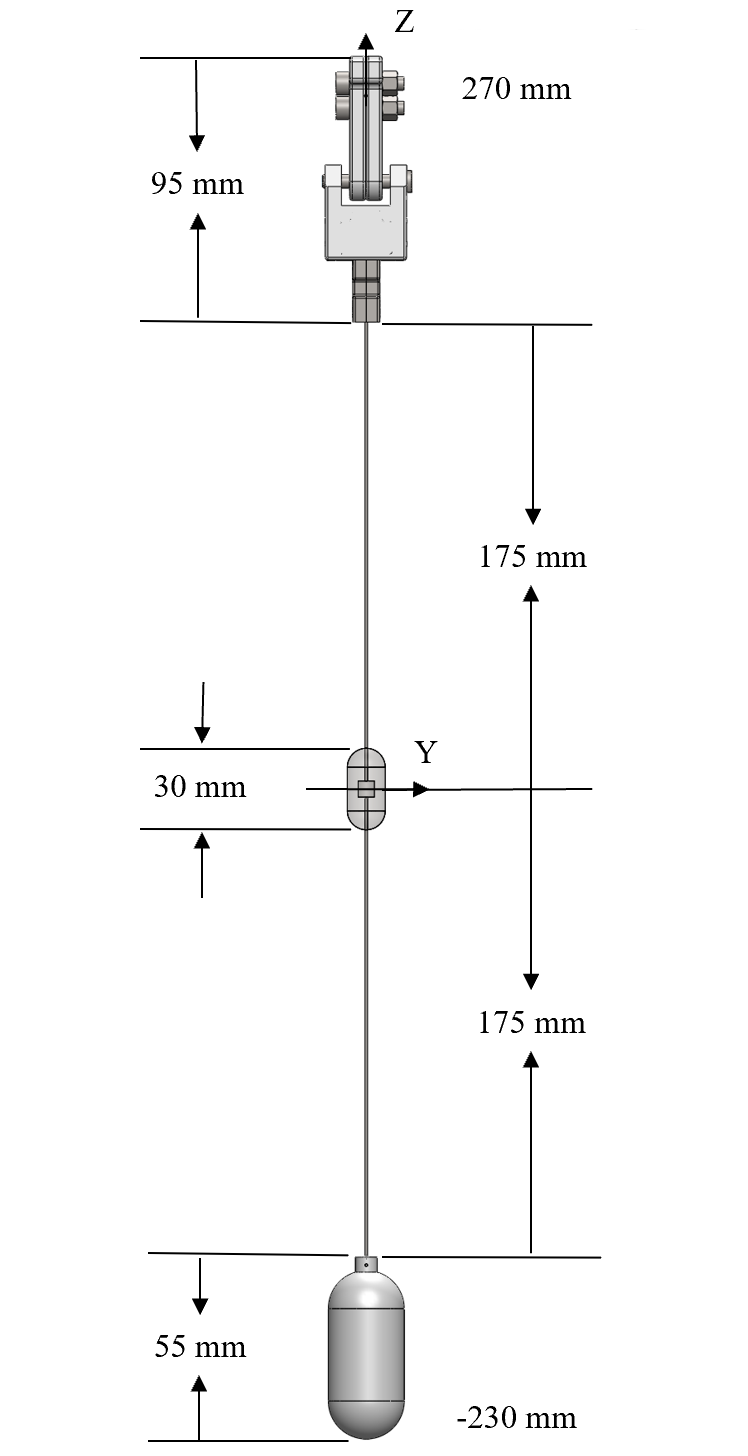
\includegraphics[width=0.7in]{source_weight_QC.png}
  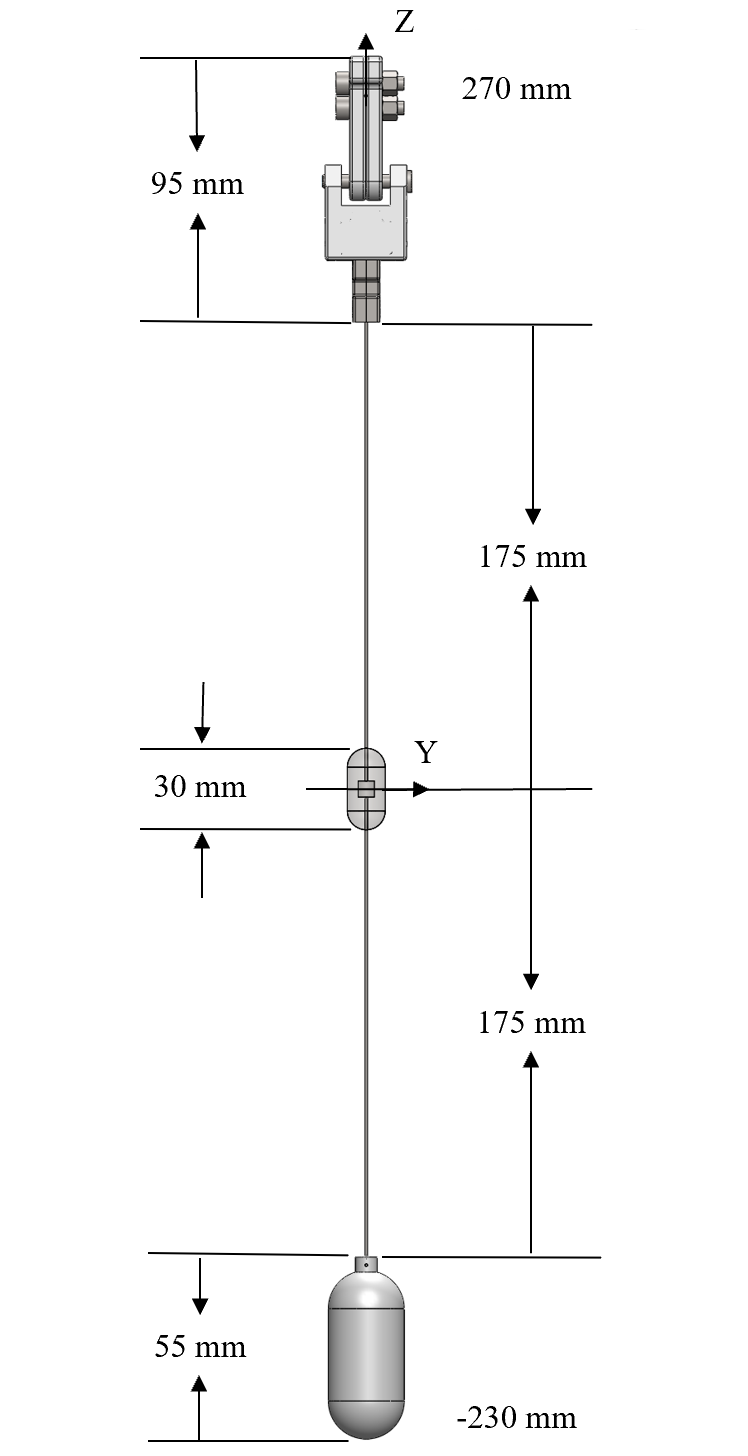
\includegraphics[width=1.2in]{source_weight_QC.png}
  \figcaption{Design of a typical source assembly. See text for
    details.}
  \label{source_weight_QC}
\end{center}
The resulting bias in
comparison to the bare sources are shown in Fig.~\ref{shadowing}, which is
less than 0.15\% for all sources. The increase of the bias toward
lower energy is expected due to the photon loss on the source shell,
and the grow toward higher energy is due to more shadowing effect on
the weight/connector.


\begin{center}
	\centering
	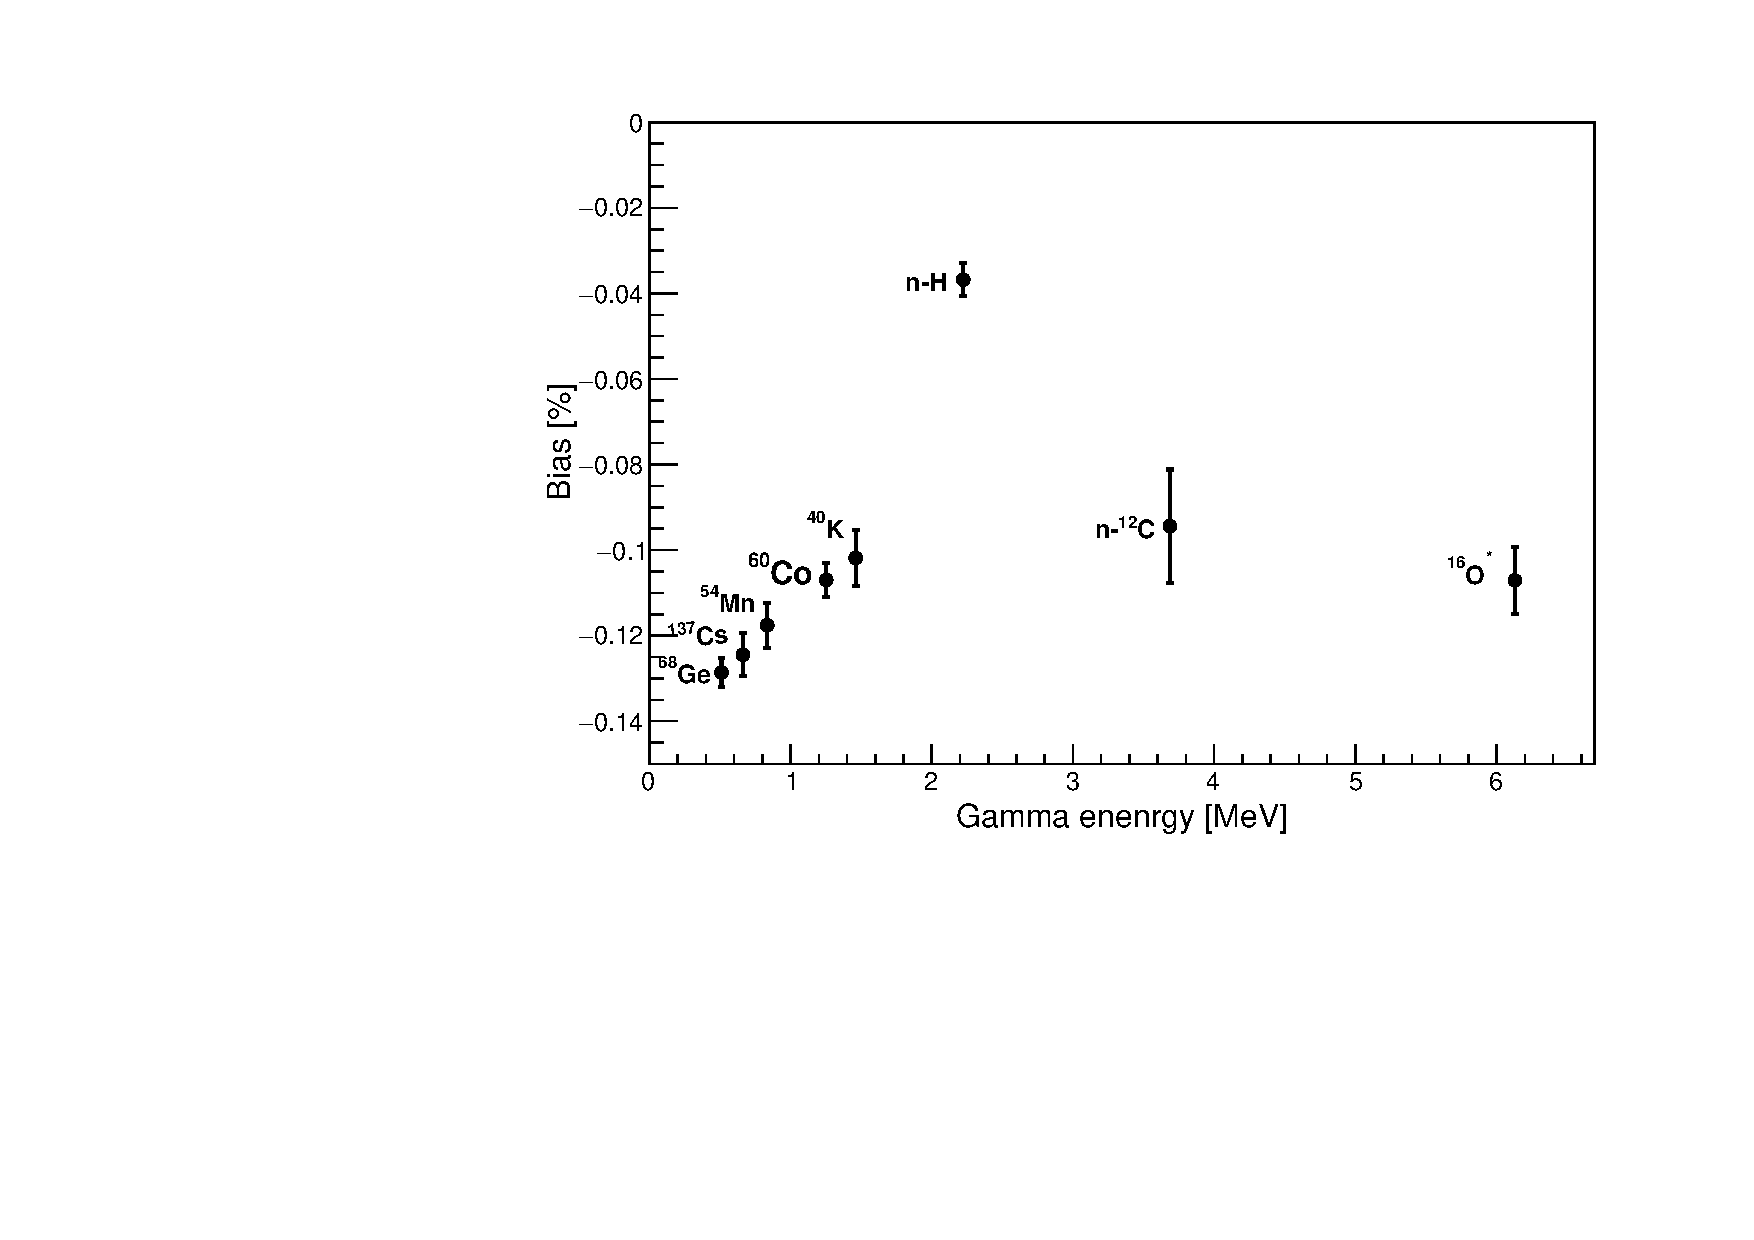
\includegraphics[width=3in]{Bias_Shadowing.pdf}
	\figcaption{Bias due to optical shadowing for individual gamma
          sources.  }
	\label{shadowing}
\end{center}

\subsubsection{Energy loss effect}
\label{sec:eloss}
Some gamma energy can also deposit in the non-scintillating material,
e.g. the enclosure of the source, leading to a leakage tail in the
detected PE spectrum. The bias to the peak is referred to as the
energy loss effect. As an example, the measured PE spectrum from the
LPMTs for a realistic $^{60}$Co source is shown in Fig.~\ref{Co60}, in
which contributions from the fully absorbed peak and the leakage tail
are separately plotted. 
\begin{center}
	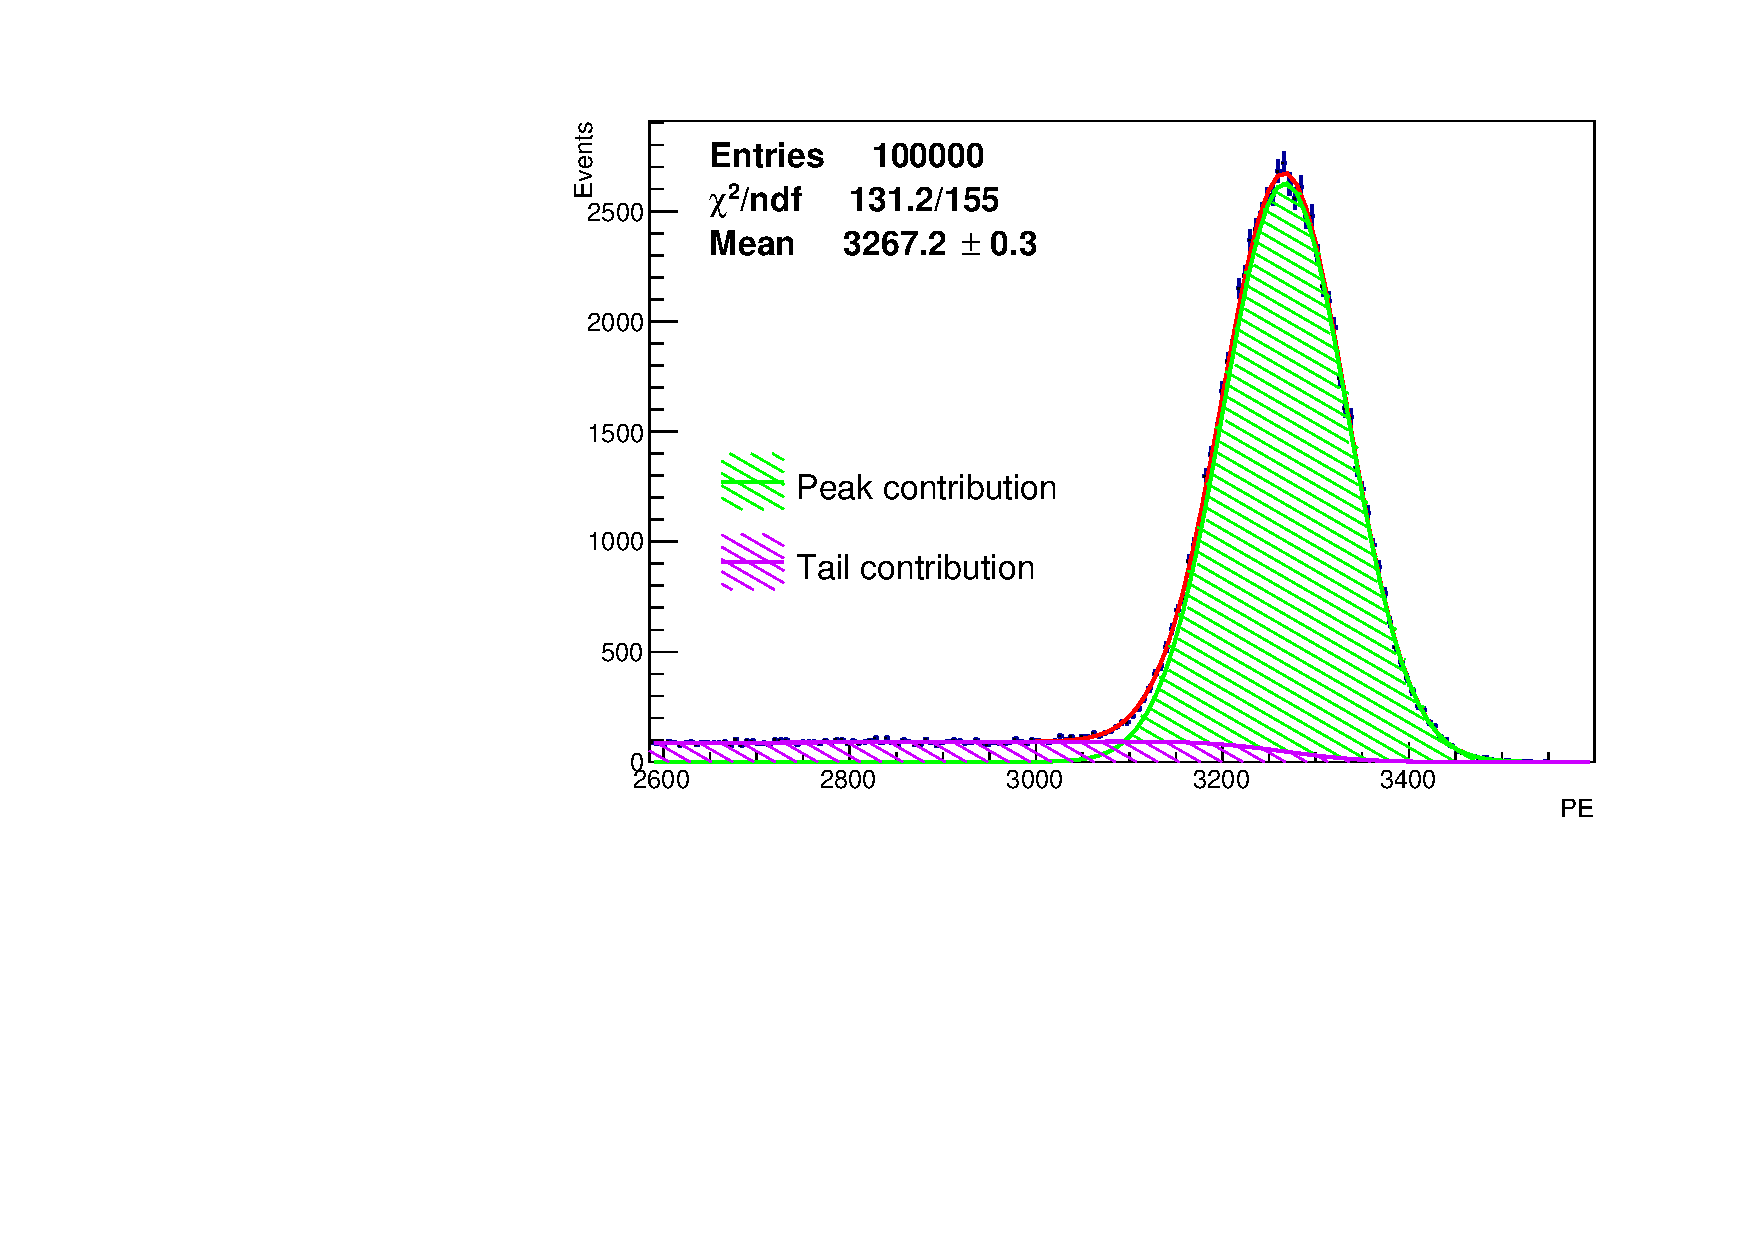
\includegraphics[width=3in]{Co60result_emc.pdf}
	\figcaption{The PE distribution of $^{60}$Co source at the
          center of JUNO. Contributions from the fully absorbed events
          and energy loss tail are indicated in the figure. See
          Sec.~\ref{sec:eloss} for details.}
	\label{Co60}
\end{center}
A fitting function with the energy loss effect taken into
account~\cite{fitmethod} is adopted here to fit the simulated gamma
spectra. The fractional difference of the best fit peak to those from
the fully absorbed events are shown in Fig.~\ref{compton}, where
residual biases are less than 0.1\% for all sources.

\begin{center}
  \centering
  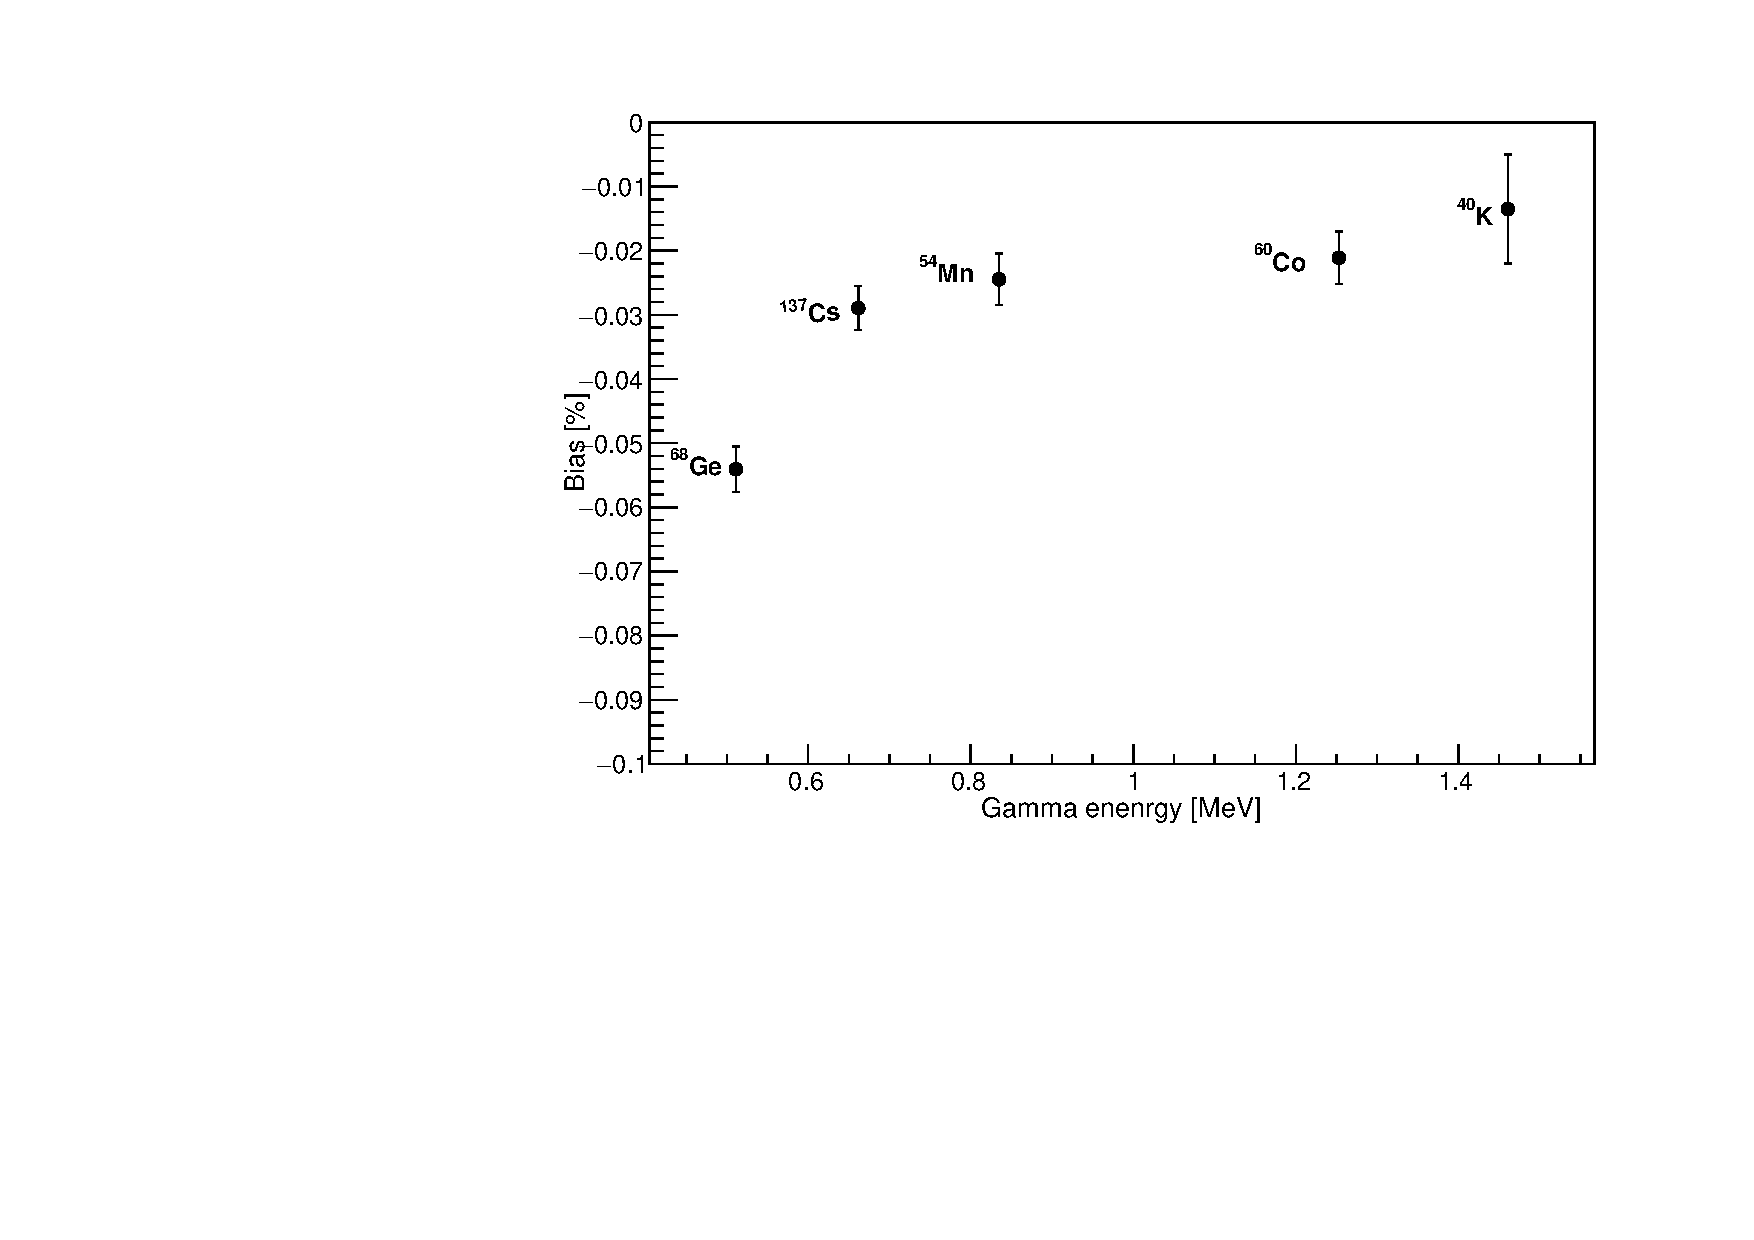
\includegraphics[width=3in]{Bias_Compton.pdf}
  \figcaption{Residual fit bias due to the energy loss effect for the
    gamma sources. Effects for higher energy gamma sources are
    negligible, so they are omitted from the figure.  }
  \label{compton}
\end{center}

\subsubsection{PMT dark rate}
\label{sec:dark_rate}
Assuming an average dark rate of 30~kHz per LPMT channel, and a 350~ns
readout time window, the dark rate pileup in any given physical event
is estimated to be 189 PE.
%$\Delta Q_{\rm DR} = 30\times10^{3}\times350\times10^{-9}\times18000=189$~PE. 
Such an offset in energy can be precisely calibrated using random triggers and
subtracted. The contribution of this pileup to the energy resolution
shall be discussed in Sec.~{\ref{sec:resolution}}.

\subsubsection{High energy gamma uncertainty}
\label{sec:uncer_highE}
High energy gammas are essential to calibrate the electron
nonlinearity at the high energy end. Such gammas can be produced via
the ($\alpha$, n) reaction when the daughter nucleus de-excites. For
example, the $^{241}$Am-$^{13}$C source can produce a 6.13 MeV gamma,
but mixed with some nuclear recoil energy. According to the SNIPER
simulation, the positive bias caused by the nuclear recoil is at a
0.4\% level. Although subtractable, this leads to a scale uncertainty
at the high energy end.

\subsubsection{Instrumental nonlinearity}
%Modification RED (previous text) and BLUE (new text)
  As discussed in Sec.~\ref{sec:elec_nonlin}, the dual
  calorimetry technique in combination to the UV laser source in
  Ref.~\cite{zhangyuanyuanpaper} and the radioactive sources is
  expected to provide a direct and clean measurement of the
  instrumental nonlinearity.  The integral nonlinearity control is
  expected to be $\leq$0.3\%, as shown in
  Fig.\ref{fig:inst_nonlinearity}, although 0.1\% accuracy seems
  possible.  This uncertainty is propagated as a fully correlated
  uncertainty in energy, but fully uncorrelated to the position
  dependent effect (next). 

\subsubsection{Position dependent effect}
\label{sec:position_dep_bias}
Since IBDs are detected throughout the detector, position dependent
energy scale variation has to be corrected for. 
The impact of this correction on the energy resolution will be elaborated in Sec.~{\ref{sec:resolution}}.
%where the residual uncertainty of less than xx\% is found. 
As we will show there, the mean scale
bias after this correction is reduced to a 0.3\% level, which is
conservatively taken as a fully correlated uncertainty in energy.

\subsubsection{Statistics}
The statistical uncertainty of the gamma peak determination is driven
by the number of calibration events. Based on fits as in
Fig.~\ref{Co60}, we validate that with 100,000 events, statistical
uncertainties of all sources can be controlled to a 0.01\% level, in
agreement with the naive estimate.

\subsubsection{Estimate of combined systematic uncertainty}
The effects discussed above are summarized in
Table~\ref{summary_uncertainty}. We assume that all the systematic can
be corrected for, but with 100\% uncertainty. We further separate the
uncertainties either into correlated in different energy, or point-to-point (single
point), depending on how they would drive individual energy
points. For example, the uncertainties due to the shadowing effects
are correlated among difference sources.

\end{multicols}

\begin{center}
	\tabcaption{A summary of the energy scale uncertainties.}
	\footnotesize
	\begin{tabular*}{170mm}{@{\extracolsep{\fill}}cccc}
          \toprule source & correction & uncertainty & nature\\
          \hline
          shadowing effect & $+$0.1\% - $+$0.2\% & correction & correlated \\
          energy loss effect & $+$0.05\% - $+$0.1\% & correction  & correlated \\
          high energy gamma uncertainty & $-$0.4\% & correction & single point (6.13 MeV) \\
          instrumental nonlinearity & n/a & (0.1,0.3]\% & correlated\\
          position dependent effect & $-$0.3\% & correction & correlated\\
          statistics & n/a & 0.01\% & point-to-point\\ 
          \bottomrule  % ???
          \label{summary_uncertainty}
	\end{tabular*}
      \end{center}

\begin{multicols}{2}

  To evaluate the combined effects, we produce toy data by randomly
  biasing the naked source values in Fig.~\ref{non_linearity_fit}
  according to the 1$\sigma$ uncertainties in
  Table~\ref{summary_uncertainty}, either in a correlated or
  point-to-point fashion. Except for the instrumental nonlinearity and
  the statistics in peak fitting, 
  %all other biasings are assumed to be one-directional, opposite to the correction. 
  all uncertainties are equal to the absolute value of the correction.
  For each set of the toy
  data, a fit as in Sec.~\ref{sec:nonlin} is performed, yielding an
  electron nonlinearity curve. This is repeated many times. The
  1$\sigma$ distribution of these fitted models are overlaid in
  Figs.~\ref{non_e_linearity_fit}
  and~\ref{fig:positron_nonlinearity}. The uncertainty band is more
  significant
  ($\sim$0.6\%)
  across all energy, so the 1\% JUNO requirement is safely satisfied.
  %at the high energy due to limited source
  %coverage and the nuclear recoil uncertainty (AmC). Nevertheless, the
  %1\% JUNO requirement is safely satisfied.

\section{Minimizing the energy resolution}
\label{sec:resolution}
Another key aspect of the calibration is to minimize the energy
resolution for the IBD positron signals. In general, the fractional
energy resolution for an average visible energy $E_{\rm vis}$ in MeV can
be written as an approximate formula
\begin{eqnarray}
  \label{eq_resolution}
  \frac{\sigma_{E_{\rm vis}}}{E_{\rm vis}}=\sqrt{\left(\frac{a}{\sqrt{E_{\rm vis}}}\right)^{2}+b^{2}+\left(\frac{c}{E_{\rm vis}}\right)^{2}}\,.
\end{eqnarray}
The $a$ term is the statistical term, which is mainly driven by the
Poisson statistics of true PEs associated with $E_{\rm vis}$.  $c$
term represents the contribution of a background noise term, i.e. the
dark noise from the PMTs, which is always mixed with $E_{\rm vis}$ in
the measurement. To set the scale, since the light yield for JUNO is
approximately $Y_0 = 1345$~PE/MeV, $a$ is about 2.7\%. As mentioned in
Sec.~\ref{sec:dark_rate}, dark rate induced energy bias is
approximately $\Delta Q_{\rm DR}\sim189$~PE, so $c$ is estimated to be
$\sqrt{\Delta Q_{\rm DR}/Y_0^2}=1.0$\%. $b$ is a constant term independent of
the energy, and in the case of JUNO, dominated by the position
non-uniformity. In Fig.~\ref{PE_vs_R}, the average number of PE for
the 511~keV gamma pairs vs. radius is shown for a few representative
$\theta$ angle in spherical coordinate. Starting from the detector
center, the gradual increase is a combined effect of due to variations
in photon coverage and attenuation. The sharp decrease close to 15.5~m
is due to the mismatch of the indices of refraction between the
acrylic and water - the closer the event to the edge, the more likely
the total reflections and consequently the losses of photons. Within
the same radius, there is an additional dispersion in $\theta$ due to
geometrical and optical complications.  The $b$ term estimated from
Fig.~\ref{spline_function} is 6\%, but can be largely removed with
calibration.

\begin{center}
        \centering
        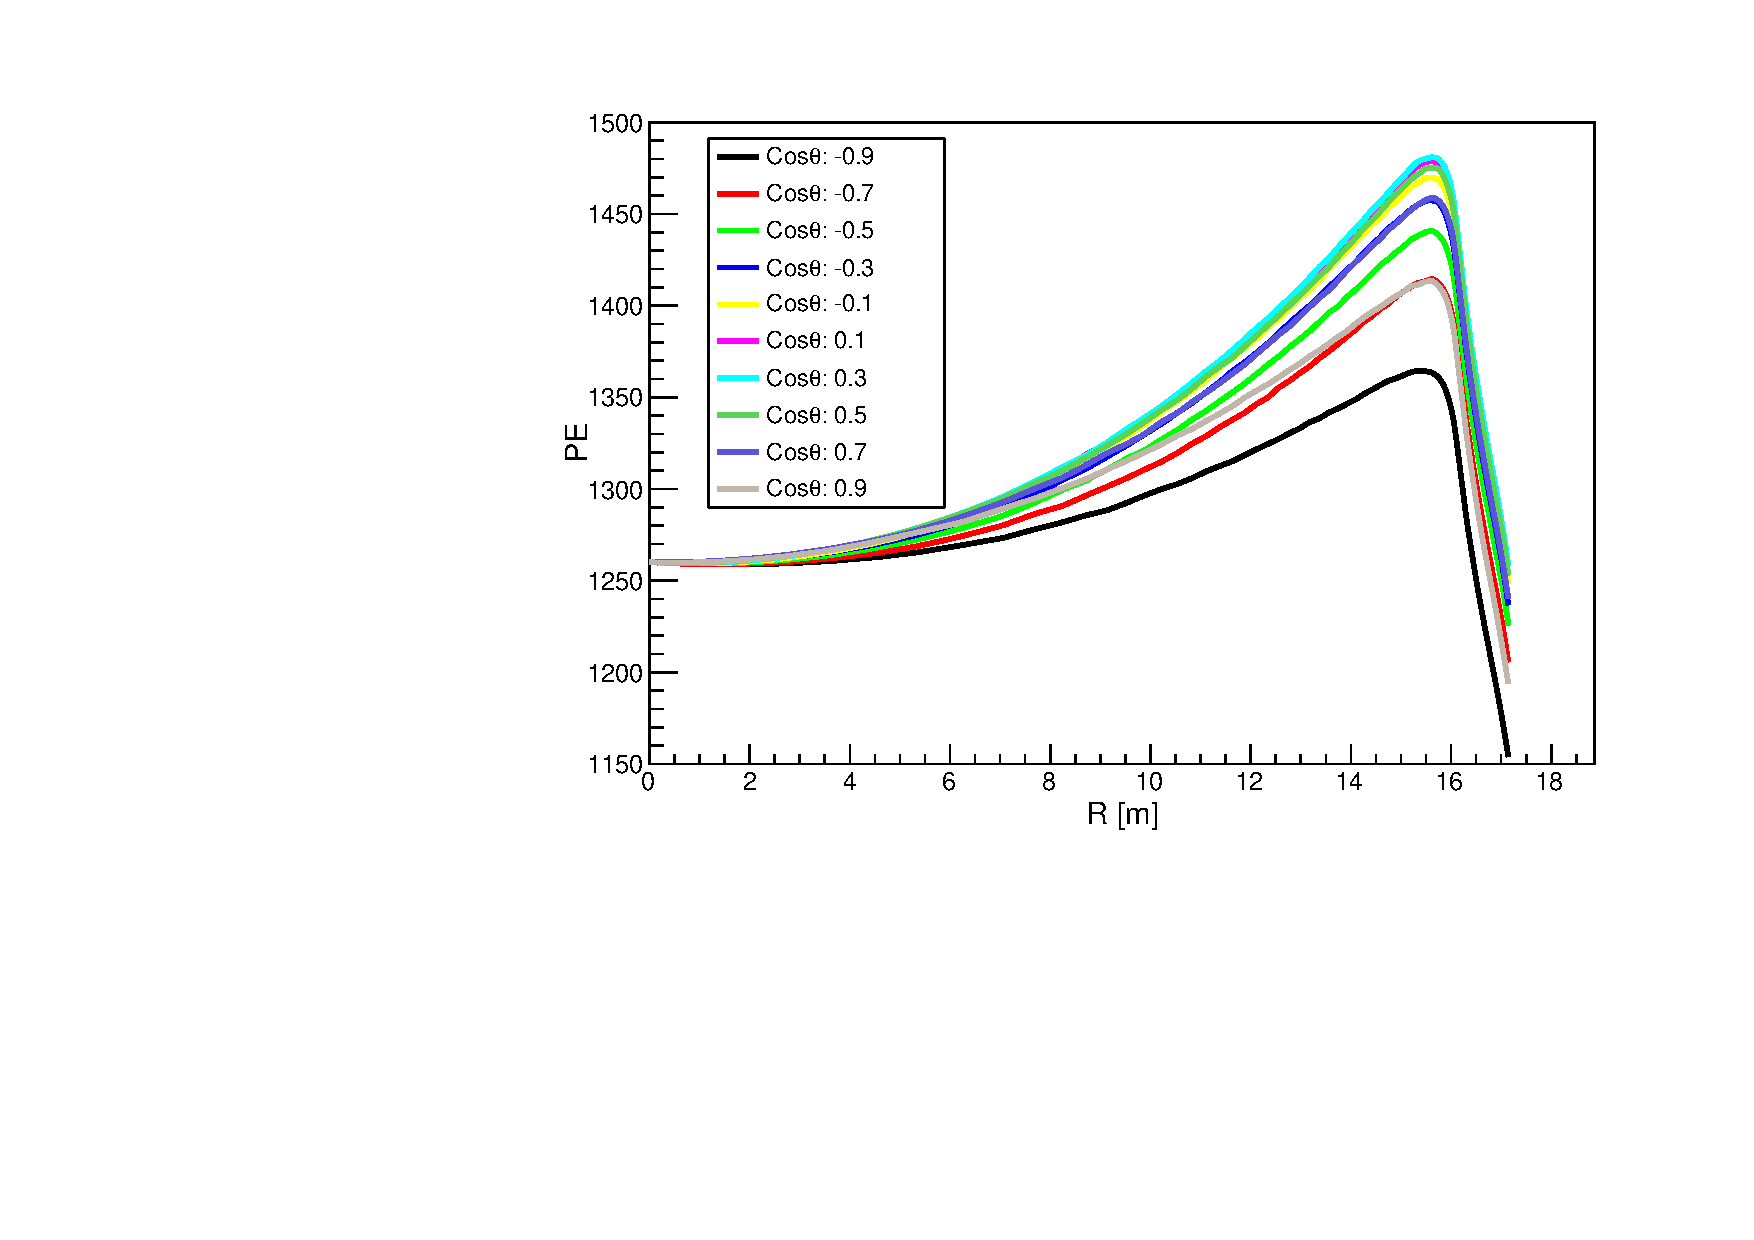
\includegraphics[width=3in]{PE_vs_R.pdf}
        \figcaption{Mean number of PEs for the 511 keV pairs as
          functions of radius, along a few representative polar angles
          (see legend).}
        \label{PE_vs_R}
\end{center}

The impact of the energy resolution (Eqn.~\ref{eq_resolution}) is
studied in details in Ref.~\cite{yellow-book}. It was found,
numerically, that the JUNO baseline requirement that the difference in
the correct and wrong hierarchy fits of the neutrino energy spectrum
reaches a $\Delta\chi^2>11$ in six years, could be translated into a convenient
requirement on an equivalent resolution term $\tilde{a}$, 
\begin{eqnarray}
\label{eq_overall_res}
\tilde{a} \equiv \sqrt{(a)^{2}+(1.6 \times b)^{2}+\left(\frac{c}{1.6}\right)^{2}} \leqslant 3 \%\,.
\end{eqnarray}
Conceptually, the facts that the constant $b$ term is not improving
with detected energy, and that the contribution of the dark noise
declines quickly with the energy, are reflected in factors 1.6 and
1/1.6, respectively. Note also that $\tilde{a}$ is only an effective
parameter, and is not the detector energy resolution at 1 MeV.

\subsection{Reducing $b$ term: non-uniformity correction}
\label{sec:non-uni}
Two complementary approaches can be used in characterizing the
detector non-uniformity, a) to deploy radioactive sources in many
locations in the detector, and b) to use uniformly distributed
background events, e.g. spallation neutrons
($\sim$1.8~evt/s~\cite{yellow-book}). Although we focus on the first
approach in this paper, it should be emphasized that the second
approach would offer a powerful {\it in situ} cross check in the real
experiment.

We define a non-uniformity function $g(r,\theta,\phi)$ as the light
yield in a given position relative to that at the center.  Ideally, to
calibrate $g$, one would like to sample as many points, in particular
in locations where it varies quickly. Practically, however, our goal
is to use finite calibration points to find a sufficiently good
approximation. To study this, simulated data are produced using SNIPER
with mono-energetic positrons from 0 to 8~MeV, uniformly distributed in
the detector. Dark rate pileup is included as an independent
Poisson-fluctuated offset with a mean value of 189 PE
(Sec.~\ref{sec:dark_rate}). The visible energy in MeV for each event
is estimated as
\begin{equation}
\label{eq_E_rec}
E_{\rm vis} = ({\rm PE_{\rm tot}}-\Delta Q_{\rm DR})/Y_0/g(r,\theta,\phi)\,.
\end{equation}
In this study, $g(r,\theta,\phi)$ is systematically stepped down from the most
complete knowledge to approximate models that we envision to obtain
through calibration. After getting the resolution at each energy,
($a$, $b$, $c$) can be extracted and compare to the requirement in
Eqn.~\ref{eq_overall_res}.

\subsubsection{Center IBDs}
In this case, all positrons are produced at the center of the
CD. Although the average light yield is slightly less in comparison to
the full volume (Fig.~\ref{PE_vs_R}), the position non-uniformity is
completely absent. Interestingly, a fit using Eqn.~\ref{eq_resolution}
to the energy resolution yields a non-vanishing $b=0.73\%$. $c =
1.38\%$ is also sizably larger than the naive dark rate estimate
(1.0\%).  The origins of these non-Poisson fluctuations were traced in
the simulation by switching off individual processes. The residual $b$
%is dominated by the non-isotropic Cerenkov photon emissions, leading
is dominated by absorption and reemission of Cerenkov photon, leading
to additional ``constant'' noise term in the detected PEs. 
The floor in $c$ is due to fluctuations caused by the annihilation gammas,
independent of the energy of the positrons.

\subsubsection{Ideal non-uniformity correction}
In the ideal case, uniformly distributed positrons are the calibration
itself. 
% 200*50*4 for R^3*costheta*phi, for every energy, 
% calibration events 500,0000. so 250 events/pixels
The detector is divided into 20,000 equal-volume``pixels'', and
$g(r,\theta,\phi)$ is computed in each pixel for every energy,
allowing a potential energy dependence (e.g. due to energy leakage at
the edge).
\begin{center}
	\centering
	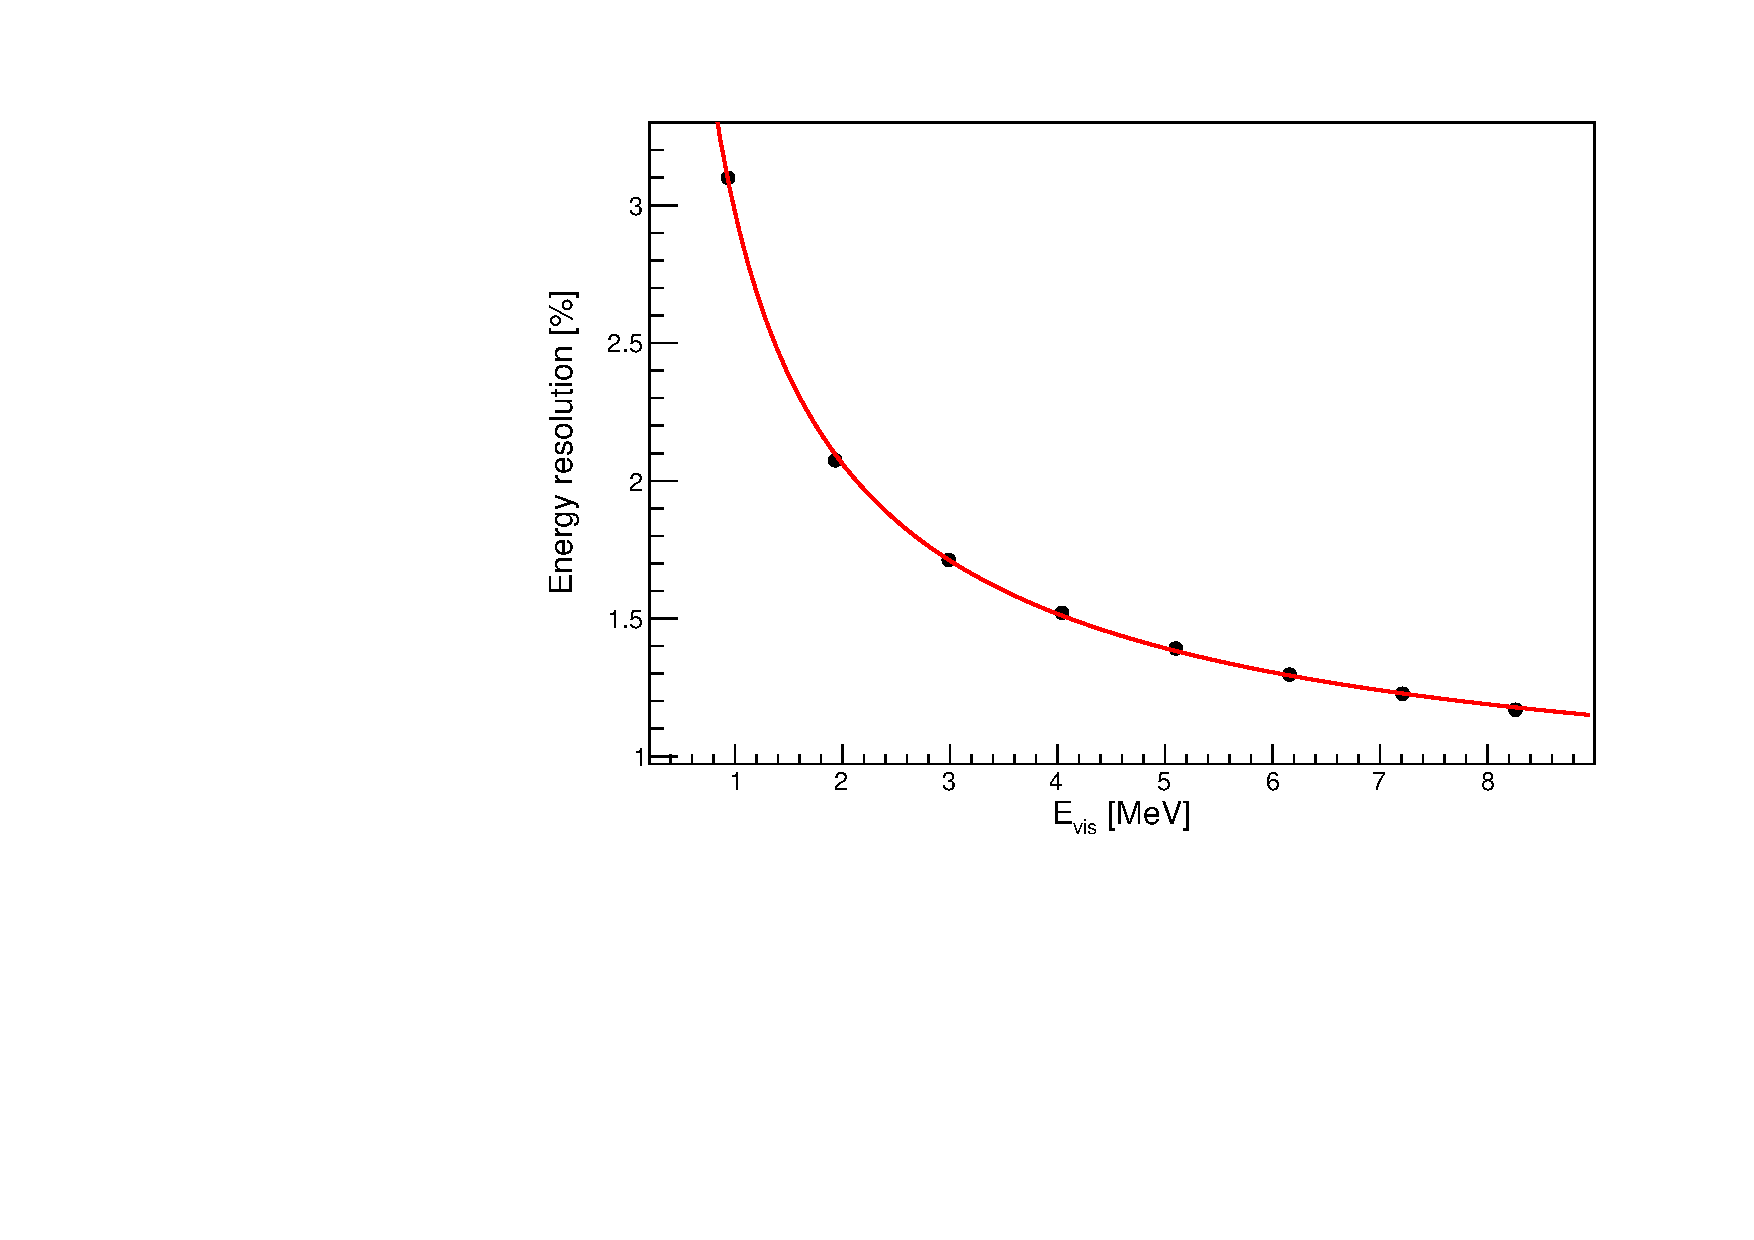
\includegraphics[width=3in]{EnergyRes.pdf}
	\figcaption{Positron energy resolution vs. $E_{\rm vis}$ after
          the ideal non-uniformity correction.}
	\label{cls_position_smearing}
\end{center}
The fit of the resolution is shown in
Fig.~\ref{cls_position_smearing}, yielding 
$a$=2.57\%, $b$=0.73\%, $c$=1.25\%, and $\tilde{a}=2.93\%$
(Table~\ref{summary_resolution}). The reductions in $a$ and $c$ terms,
in comparison to those of the center IBDs, is due to the increase of
full-volume light yield (Fig.~\ref{PE_vs_R}). This scenario should
serve as the most ideal reference for the calibration.

\subsubsection{Utilizing azimuthal symmetry}
The azimuthal symmetry in the JUNO detector allows the first
simplification, that only $g$ in a vertical half plane of the detector
is needed. For illustration, $g(r,\theta)$ surface in the $\phi=0$
plane for positrons with zero kinetic energy is shown in
Fig.~\ref{spline_function}. The two-dimensional $g(r,\theta)$ function
obtained at each positron energy is then applied to corresponding
positron events. The resulting $\tilde{a}$ is 2.96\%, a validity check
of the azimuthal symmetry assumption.
\begin{center}
	\centering
	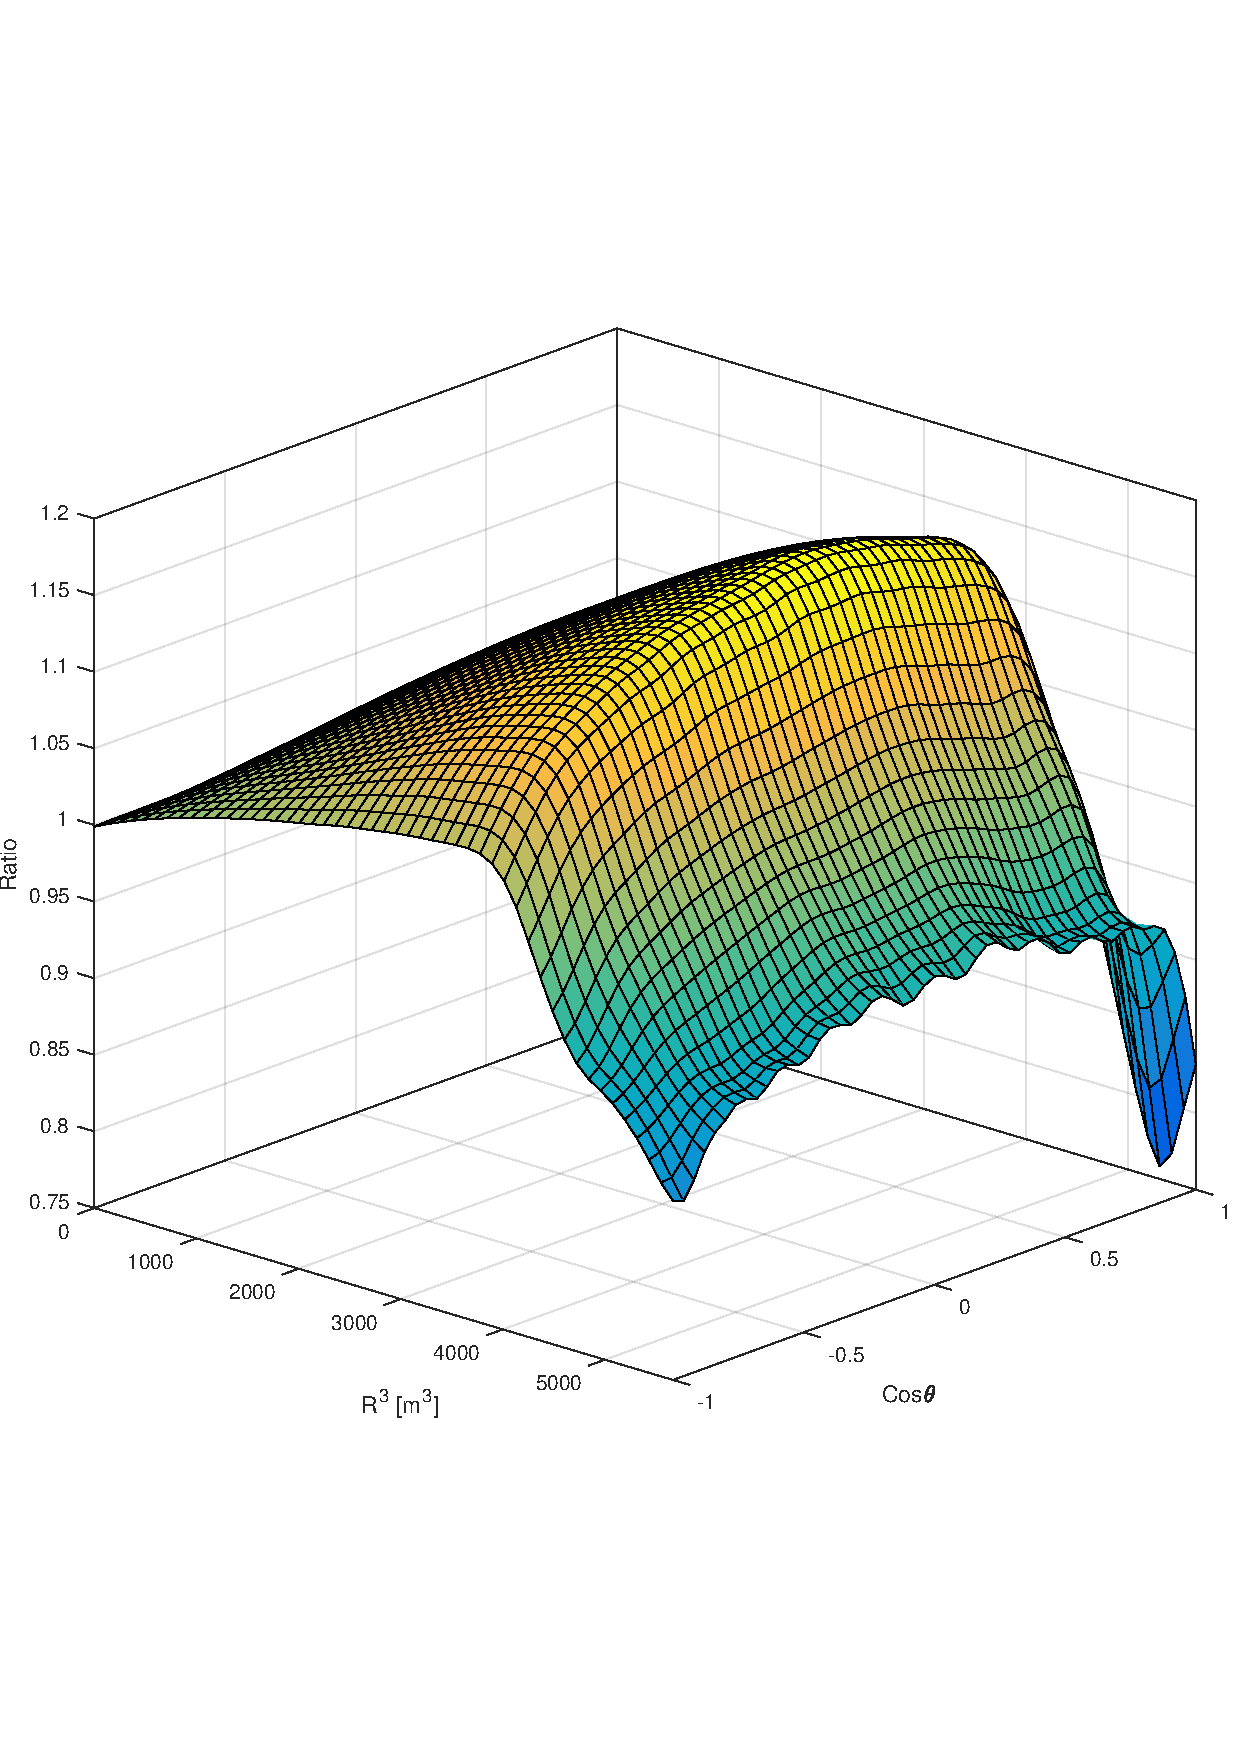
\includegraphics[width=3in]{spline_function.pdf}
	\figcaption{The non-uniformity $g$ in the $\phi=0$
          plane for 0 MeV positrons.}
	\label{spline_function}
\end{center}

\subsubsection{Single gamma source}
One more step towards the reality is to use a single gamma line to
replace $g(r,\theta)$ obtained by the hypothetical positron
sources. We choose the 2.22 MeV neutron-proton capture gammas to allow
direct comparisons to the spallation neutron capture signals in the
real experiment, and to minimize the source shadowing effects
(Fig.~\ref{shadowing}). After the application of this $g(r,\theta)$,
$\tilde{a}$ is 2.98\%. This also implies that the energy dependence of
$g$ can be safely omitted.

\subsubsection{Finite calibration points}
\label{finite-calib-p}
The next critical simplification is to select a list of ``must-do''
calibration points which would still give a satisfactory
correction. Several pragmatic considerations are
\begin{itemize}
\item As observed in Fig.~\ref{spline_function}, there is no apparent
  symmetry in $g(r,\theta)$ that allows a vast simplification to the
  choice of points. However, the variation of $g$ appears faster at
  the edge, which mandates more sampling points there.

%\item To constrain the spline function, the boundaries of the vertical
%  half-plane are critical, i.e. the central axis of the detector and
%  the inner circle at the LS-acrylic boundary.  The central axis can
%  be calibrated with good granuality, for example, one point per
%  meter (35 total).  The JUNO acrylic sphere is made up in 23 layers, each
%  supported by supporting fixtures with non-trivial impact to the
%  internal optics of the CD. Therefore, the acrylic boundary should be
%  calibrated at the corresponding 23 locations. 

\item To constrain the surface of $g(r,\theta)$, the boundaries of the
  vertical half-plane are critical, i.e. the central axis of the
  detector and the inner circle at the LS-acrylic boundary.  The
  central axis can be calibrated with good granularity, for example,
  one point every 2 meters for radius less than 12 m, one point every
  meter from 12 m to 17 m, and two points at 17.2 m and 17.5 m (27
  points in total).  For the acrylic boundary, the sphere is made up
  in 23 layers, each supported by SS fixtures with non-trivial
  impact to the optics. It would therefore be sensible to calibrate
  these 23 additional locations.

\item For the region in between, if we start from the 23 points at the
  acrylic boundary and calibrate 9 more points along the radial line,
  this would make roughly 200 more points. Another practical
  consideration is the duration - if time spent at each calibration
  point (including source moving time) is 5 minutes, 200 points would
  take 16 hours, a reasonable duration.

\item Realistically, not all points in $(r,\theta)$ are accessible. If
  we consider a SNO-like cable loop system~\cite{SNO} with anchors on
  the inner surface of the CD (see
  Fig.~\ref{overview_calibration_system}), some points too close to
  the vertical geometrical limits cannot be reached due to the loss of
  cable tensions (Ref.~\cite{zhangyuanyuan-new-paper}). To allow a
  good coverage we consider two cable loops
  (Figs.~\ref{overview_calibration_system}~and~\ref{basic_coverage}) in the
  CD. Note that physically the two loops can be at different vertical
  planes, and azimuthal symmetry can be applied to combine them into a
  single $(r,\theta)$ half-plane.
\end{itemize}

Given the above, the optimization of calibration points is correlated
with the choice of the two anchor locations ($\theta_1$,$\theta_2$)
for the cable loops. An automatic optimization is performed using the
following procedure. 1) We fix the 27+23 points along the two
boundaries described above, and perform SNIPER simulations with 2.22
MeV gammas. 2) We go through all possible ($\theta_1$,$\theta_2$)
combinations, each with its own accessible region in $(r,\theta)$
(Fig.~\ref{basic_coverage}). 3) For each ($\theta_1$,$\theta_2$), 200
points are randomly chosen, on which the 2.22 MeV simulations are
made. 4) For each set of 200 (random) plus 50 (fixed) points, a smooth
surface of $g(r,\theta)$ is constructed using a two-dimensional
spline function. 5) Such $g(r,\theta)$ is applied to the uniform
positron events, on which $\tilde{a}$ is extracted as a
figure-of-merit. Steps 1) through 5) are repeated until a minimal
$\tilde{a}$ is found. The final choice of the calibration points are
illustrated in Fig.~\ref{basic_coverage}, in which the best anchor
locations are $\theta_1=\ang{48}$ and $\theta_2=\ang{78}$.  The
resulting $\tilde{a}$ is 2.98\%, very similar to that obtained using
``infinite'' calibration points.

\begin{center}
  \centering
  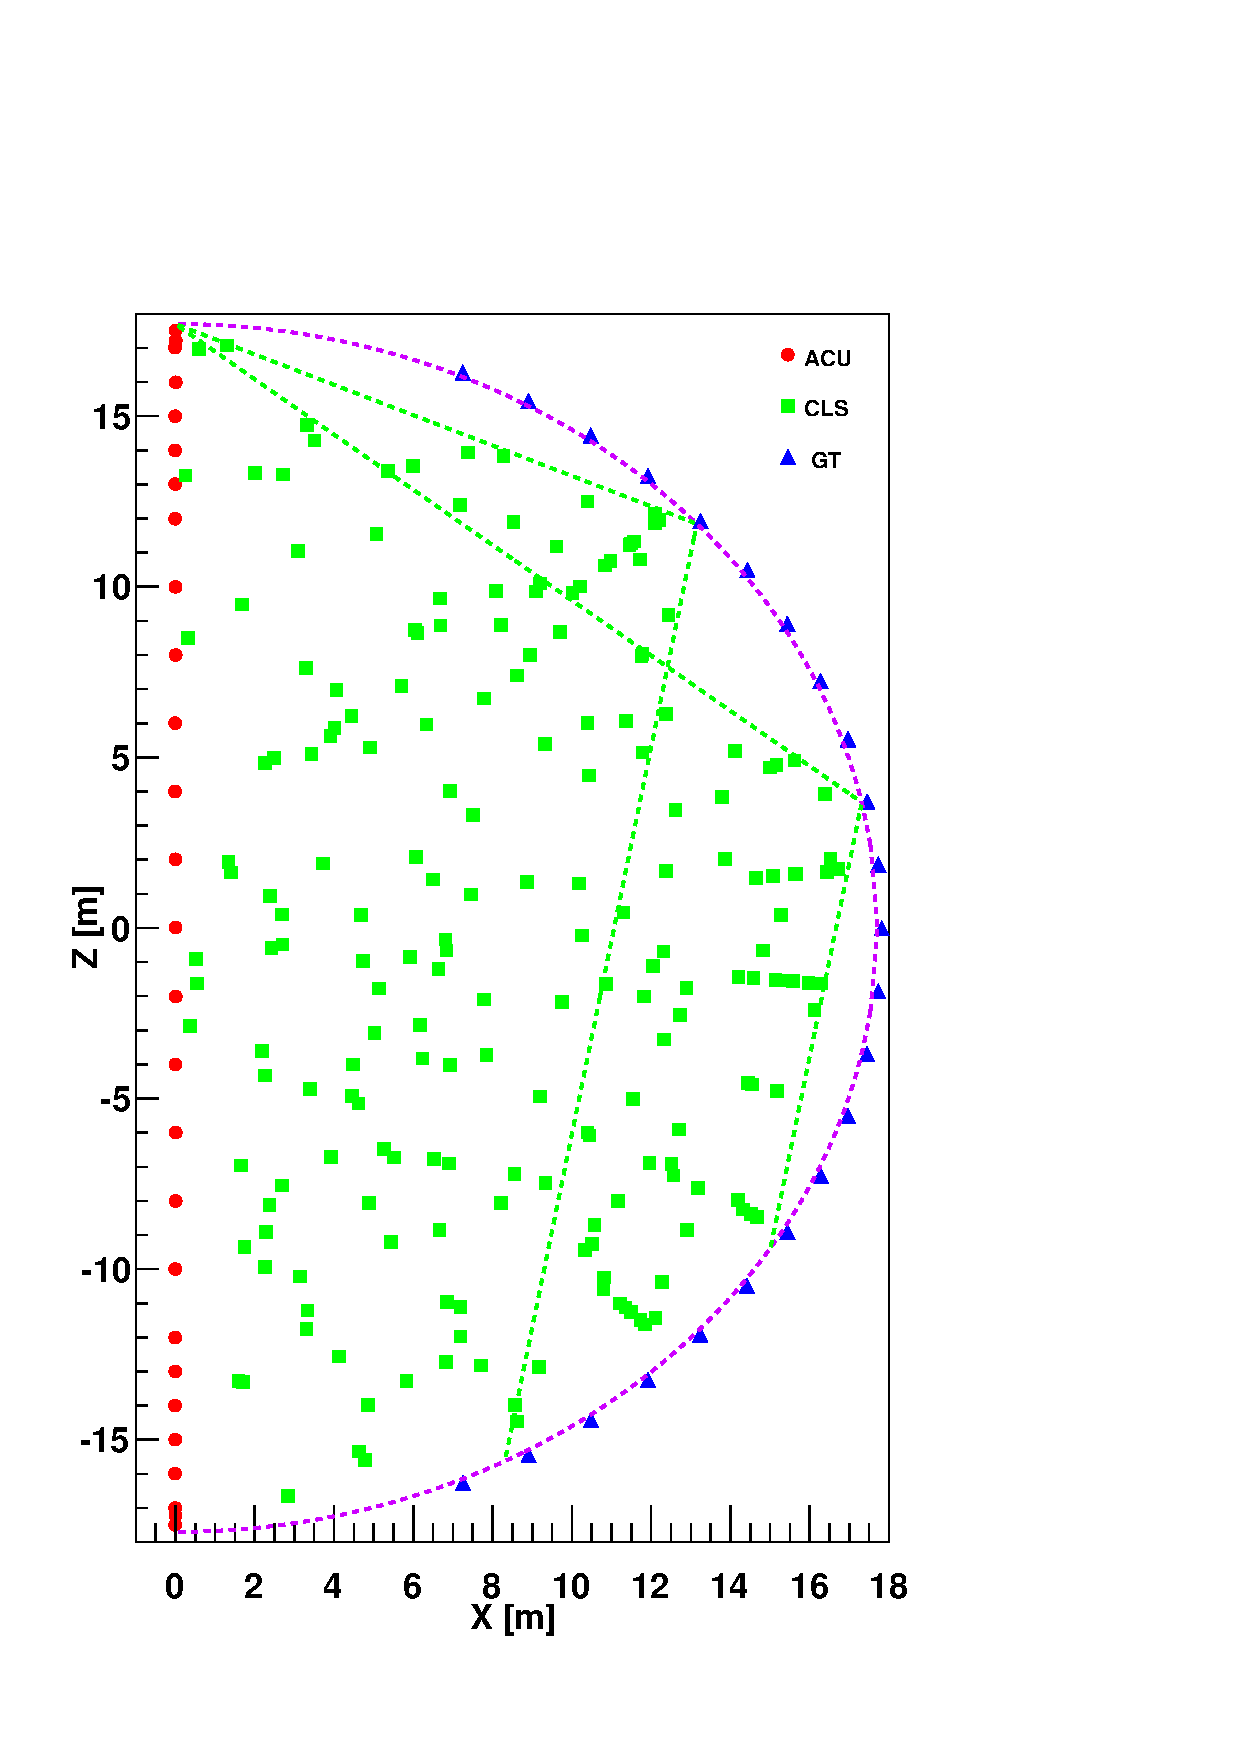
\includegraphics[width=3in]{basic_coverage.pdf}
  \figcaption{Coverage of the 250 calibration points after
    optimization. The dashed lines are the upper and assumed outer
    (\ang{10} from vertical) boundaries of the coverage of the cable
    loops.}
        \label{basic_coverage}
\end{center}

\subsubsection{Vertex smearing}
So far in making corrections to the reconstructed energy, we have used
the true vertex in looking up $g(r,\theta)$. In reality, the
event-by-event correction has to rely on the reconstructed vertex,
which will in turn affects the quality of the correction.  An
algorithm based on time and charge information of LPMTs have been
developed in Ref.~\cite{vertex-rec} where a resolution of
8/$\sqrt{E(\rm{MeV})}$~cm (average distance between the true and
reconstructed vertex) was achieved. To study the impact to the overall
resolution, we study three assumptions here, 8/$\sqrt{E(\rm{MeV})}$,
10/$\sqrt{E(\rm{MeV})}$, and 15/$\sqrt{E(\rm{MeV})}$~cm. For each
simulated event, position smearing is made accordingly before applying
$g(r,\theta)$ in Sec.~\ref{finite-calib-p}. The corresponding
$\tilde{a}$ is 3.01\%, 3.05\%, and 3.1\%, respectively.

Another related effect is that we only know the calibration source
location to certain precision, leading to a small smearing
to $g(r,\theta)$. The hardware requirement is a precision of
3~cm~\cite{JUNOCDR} - significantly better than the reconstructed
resolution at 1~MeV. It is verified that this contribution can be
neglected.

\subsubsection{LPMT quantum efficiency fluctuation}	
	For each LPMT, the quantum efficiency (QE) was
  measured individually in the quality assurance process with an
  average value of $\sim$30\% at 430 nm. The $1\sigma$ fractional
  variation of the QE was measured to be 7\%. Therefore, instead of a
  constant, we assumed a random variation in QE of 7\%, while keeping
  the average the same. The result is summarized in
  Table~\ref{summary_resolution}.  Due to the PMT QE fluctuation, the
  $\tilde{a}$ deteriorates from 3.01\% to 3.02\%.

\subsubsection{Realistic detector}
\label{sec:real_det}
So far we have discussed the simulation of an ideal JUNO with nominal
parameters in SNIPER. A real detector can certainly differ from the
simulation, so it is important to study whether an {\it in situ}
calibration in a realistic detector can still achieve the required
resolution. Five conservative alterations of the CD are considered:
\begin{enumerate}
\item The JUNO LPMT and readout electronics are designed to yield less
  than 1\% dead channels ($\sim$180) in six years. We assume a CD
  with 1\% LPMT failed in random positions. 
\item Same as above but forcing an additional asymmetry among the bad
  channels (75:105, $\sim$1\% cumulative binomial p value) in the two
  semispheres separated by the calibration plane
  (Fig.~\ref{basic_coverage}), breaking the assumed azimuthal
  symmetry.
\item The JUNO LS has been tested in one of the
    decommissioned Daya Bay detector for 1.5 years, so all optical
    parameters in JUNO LS are validated with this data. No temporal
    degradation of the light yield of this special detector has been
    observed with $\sim$0.5\% standard deviation among
    measurements~\cite{YuZeyuan_LSpaper}. For conservativeness, we
    still assume that the light yield of JUNO $Y_0$ is reduced by 1\%
    and 5\% and study their effects.
\item A 4\% reduction of the absorption length ($\sim$77~m at
  430~nm~\cite{JUNOLSAbsL} in SNIPER) can also produce a 1\% reduction
  of $Y_0$. However, instead of a global reduction of light yield
  everywhere, the reduction of absorption length alters the uniformity
  of the detector. We assume such scenario in the simulation.
\item The PMT resolution will also affect the
    energy resolution, if we naively use the measured charge (integral
    of the waveform) as the energy estimator. However, one should note
    that within the IBD energy range, most LPMTs are still working
    under the single photon counting regime, therefore one could use
    waveform-based photon counting analysis to avoid the resolution
    smearing. A successful application of this approach is in
    Ref.~\cite{Lux-single-photons}. A waveform deconvolution
    technique~\cite{huangyongbo-papper} may also offer a better
    estimator for number of photons. Nevertheless, we assume a 30\%
    single-photoelectron resolution for each LPMT to study the effect.
\end{enumerate}

In each case, we recalibrate using the above program, obtain the
$g(r,\theta)$ map, then apply it to uniformly distributed
positrons. The results are summarized in
Table~\ref{summary_resolution}. In the two cases
  where $\tilde a$ exceeds 3.1\% (5\% reduction of light yield, or the
  inclusion of 30\% charge resolution for each PMT), sizable increase
  of the $a$ term is observed (as expected), for which it is beyond
  the control of the calibration program. For all other cases, the
  impact of the residual $\tilde a$ is minor, indicating the
  effectiveness of the calibration program.

%the {\it in situ} calibration scheme can characterize
%the non-uniformity sufficiently well, and the resulting energy
%resolution is satisfactory.

\subsubsection{Bias in the energy scale}
  With the optimized 250 calibration points in
  Fig.~\ref{basic_coverage}, we also evaluate the residual bias in the
  energy scale. With nominal JUNO detector and the two-dimensional
  $g(r,\theta)$ above, the relative difference between $E_{\rm vis}$
  (corrected using Eqn.~\ref{eq_E_rec}) of uniform positron events to
  that at the CD center is less than 0.05\%.  For the five realistic
  detector conditions above, with the {\it in situ} calibration, the
  bias can be reduced to below 0.3\% (adding the latter
  five effects in quadrature), as shown in
  Table~\ref{summary_resolution}. This residual bias has been included
  as a systematic uncertainty in the positron energy scale in
  Sec.~\ref{sec:position_dep_bias}. 


\subsection{Conclusion of the energy resolution}
The step-by-step downgrade of the non-uniformity calibration from the
ideal to the most realistic situation is summarized
Table~\ref{summary_resolution}. One sees that the constant term $b$ in
the energy resolution can be minimized utilizing a single gamma source
with about 250 points in a vertical half plane of the CD, bootstrapped
to the entire CD using a smooth two-dimensional spline function in
$(r,\theta)$. The nominal JUNO with the above
  calibration program will lead to an $\tilde a$ of 3.02\%, in
  agreement with the requirement put forward in
  Ref.~\cite{yellow-book}. For other potential detector imperfections,
  although it is difficult to predict what may happen in a real
  detector, the individual impact can lead to a worst-case $\tilde a$ of
  3.12\%.
\end{multicols}
\begin{center}
  \tabcaption{Energy resolution after sequential downgrade from the
    ideal to realistic calibration. Values in parentheses indicate
    fitting uncertainties. For effects mentioned in
      Sec.~\ref{sec:real_det}, they are studied independently but by including all
      effects down to the PMT QE fluctuations.}  \footnotesize
  \begin{tabular*}{170mm}{@{\extracolsep{\fill}}ccccccc}
    \toprule  % ???
    Effects & $a$ & $b$ & $c$ & $\tilde{a}=\sqrt{a^{2} +(1.6b)^{2} + (\frac{c}{1.6})^{2}}$ & energy bias (\%)\\ 
    \hline
    CD center & 2.62(2) & 0.73(1) & 1.38(4) & 2.99(1) & - \\
    Ideal correction & 2.57(2) & 0.73(1) & 1.25(4) & 2.93(1) & - \\
    Azimuthal symmetry & 2.57(2) & 0.78(1) & 1.26(4) & 2.96(1) & - \\
    Single gamma source & 2.57(2) & 0.80(1)& 1.24(4) & 2.98(1) & - \\
    Finite calibration points & 2.57(2) & 0.81(1)& 1.23(4) & 2.98(1) & - \\
    Vertex smearing(8 cm) &2.60(2) & 0.82(1) & 1.27(4) & 3.01(1) & - \\
    PMT QE fluctuation & 2.61(2) & 0.82(1) & 1.23(4) & 3.02(1) & 0.03(1)\\\hline
    1\% PMT death (random)&2.62(2) & 0.84(1) & 1.23(5) & 3.04(1) & 0.09(1) \\
    1\% PMT death (asym) &2.63(2) & 0.86(1) & 1.20(4) & 3.06(1) & 0.23(1) \\
    $Y_0$ reduced by 1\% & 2.62(2) & 0.85(1) & 1.25(4) & 3.05(1) & 0.09(1) \\
    $Y_0$ reduced by 5\% & 2.68(2) & 0.85(1) & 1.28(5) & 3.11(1) & 0.09(1) \\
    Absorption length reduced by 4\% &2.62(2) & 0.82(1) & 1.27(4) & 3.03(1) & 0.07(1)\\
    PMT charge resolution (30\%) &2.72(2) & 0.83(1) & 1.23(5) & 3.12(1) & 0.08(1) \\
    \bottomrule  % ???
    \label{summary_resolution}
  \end{tabular*}
\end{center}
\begin{multicols}{2}

\section{Conceptual design of the calibration system}
\label{sec:CalibSys}
The hardware design of the calibration system is mostly driven by the
non-uniformity calibration requirements. As demonstrated in
Sec.~{\ref{sec:resolution}}, such a system should be capable to deliver
a source along the central axis of the CD, the circle at the
LS-acrylic boundary, and the region in between. The corresponding
hardware design consists of several independent subsystems
(Fig.~\ref{overview_calibration_system}), which will be discussed in
turn.

\begin{center}
  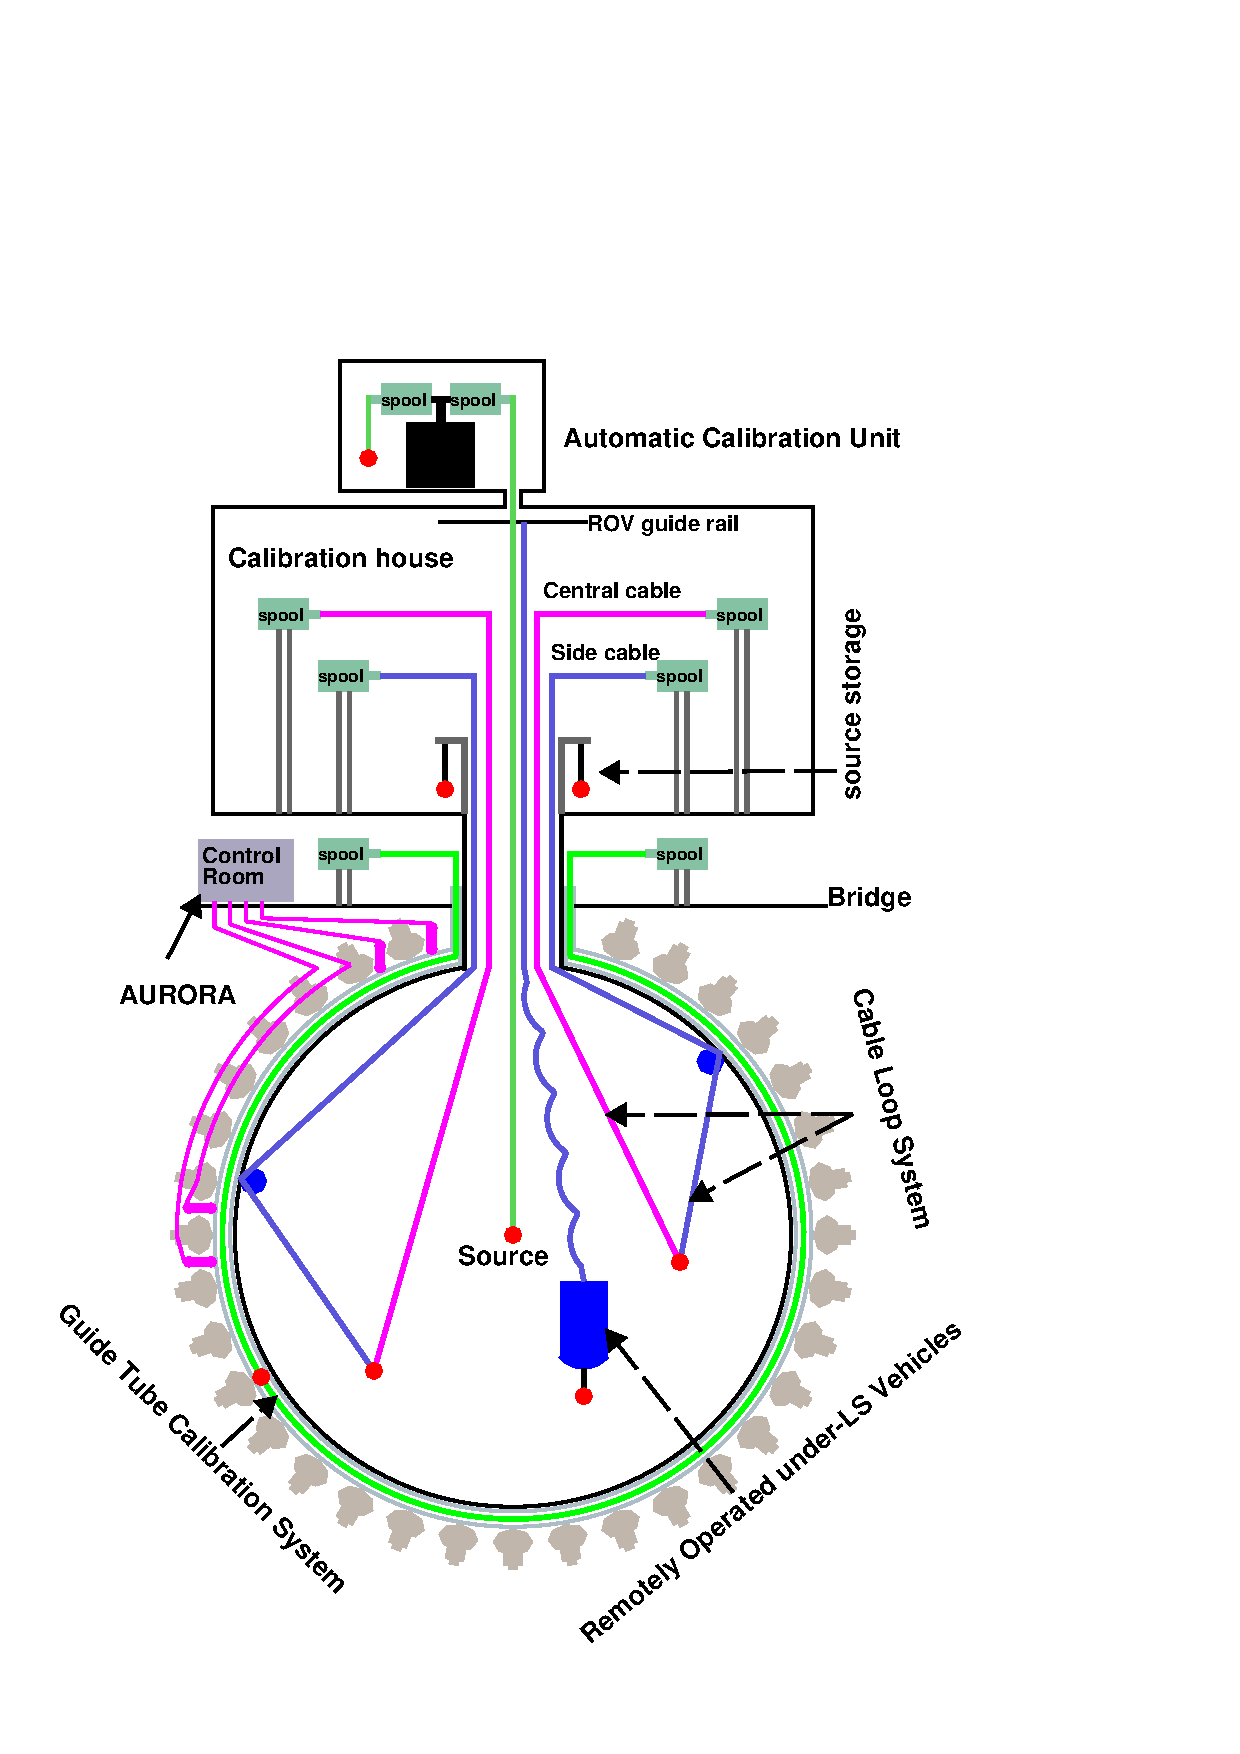
\includegraphics[width=2.5in]{calib_systems.pdf}
  \figcaption{Overview of the calibration system (not drawn to scale),
    including the ACU, two CLSs, the GT, and the ROV. The AURORA is a
    auxiliary laser diode system to monitor the attenuation and
    scattering length of the LS, which is beyond the scope of this
    paper.}
  \label{overview_calibration_system}
\end{center}

\subsection{Automatic calibration unit (ACU)}
The ACU is developed to do calibration along the central axis of the
CD. The design is very similar to the ACU in the Daya Bay
experiment~\cite{dayabayACU}, with four independent spools mounted on
a turntable. Each spool is capable to unwind and deliver the source
under gravity through the central chimney of the CD, with a high
positioning precision ($\sim$cm). Three sources can be deployed
regularly, including a neutron source (AmC), a gamma source
($^{40}$K), and a pulsed UV laser source carried by an optical fiber
with a diffuser ball attached to the end. To be flexible, the fourth
spool will carry a replaceable source, for example a radioactive
source or even a temperature sensor. Due to its simplicity and
robustness, we envision to use it frequently during data taking to
stabilize the energy scale, and to partially monitor the position
non-uniformity.

\subsection{Guide tube system (GT)}
The GT is a tube looped outside of the acrylic sphere along a
longitudinal circle. Within the tube, a radioactive source with cables
attached to both ends gets driven around with good positioning
precision. The design of this system is discussed in details in
Ref.~\cite{GTCS}. Although physically outside of the CD, MeV-scale
gammas can easily penetrate the 12~cm acrylic and deposit energy into
the LS, despite that the full absorption peak is mixed with a somewhat
significant leakage tail (correctable by fitting). Based on the
simulation studies in Ref.~\cite{GTCS}, this subsystem is sufficient
to calibrate the CD non-uniformity at the boundary.

\subsection{Cable loop system (CLS)}
As illustrated in Fig.~\ref{overview_calibration_system}, two CLSs
lying in the two opposite half-planes serve the source deployment in
off-axis positions. For each CLS, two cables are attached to the
source, which also forms a loop to deliver and retract the source. The
center cable goes upwards towards the chimney of the CD. The side
cable winds through an anchor on the inner surface of the acrylic
sphere, then towards the north pole of the CD, then vertically upwards
through the chimney as well. By adjusting the lengths of the two
cables, the source ideally could be delivered within an area bounded
by the vertical lines through the anchor and the central axis. More
realistic coverage measured by a CLS prototype will be reported in a
separate paper~\cite{zhangyuanyuan-new-paper}. Two CLSs with anchors at
different polar angles allows a better coverage of the full
half-plane, assuming an azimuthal symmetry. The overlapping points
also allow direct checks on the azimuthal symmetry. In
Sec.~\ref{finite-calib-p}, the optimized polar angles of the two
anchors have been determined to be \ang{48} and \ang{78}.

\subsection{Remotely operated under-LS vehicles (ROV)}
Locations other than the CLS plane could also turn out to be
important, if there are significant local effects which break the
azimuthal symmetry. These locations can be accessed by physical
background events, for example, the spallation
neutrons. Alternatively, we also plan to have a ROV similar to that in
the SNO experiment~\cite{SNO-ROV}, capable to deploy a radioactive source
in the entire LS volume. Such a ROV needs to work with an independent
positioning system. The mechanical design also needs to be optimized
in size and surface reflection to minimize the loss of
photons. Cleanliness control both in radioactive and chemical
contaminations to the LS is another key design consideration. We
envision that the ROV serves as a supplement of the ACU, CLS, and GT,
and should be deployed very infrequently.

\subsection{Positioning system}
For the four subsystems above, ACU and GT have good positioning
controls through accurate measurements of the cable lengths. For the
CLS, due to friction in the loop and the self-weight of the cable,
realistic cables do not run in straight lines. Therefore,
calculations based on naive trigonometric relations introduce
significantly uncertainties in the source
location~\cite{zhangyuanyuan-new-paper}.  For the ROV, it is even more
complex as the positioning is needed during the navigation. For these
purposes, an independent ultrasonic positioning system has been
developed. Eight ultrasonic receivers will be mounted inside the
acrylic sphere, and the source deployed by the CLS or ROV will carry a
miniature ultrasonic emitter~\cite{NWPU-paper}. Based on the prototype
tests, such a system is capable to provide a positioning precision to
better than a few cm.

\section{JUNO calibration program}
\label{sec:calib_program}
Based on all discussions above, we can now streamline the calibration
program. The rates of the radioactive source are set to be around 100
neutron or gamma emissions per second (except $^{40}$K which can only
be made with natural potassium salt), so that the data rate during the
calibration does not differ too much from that during the neutrino
data taking ($\sim$1000~Hz). Under this rate, a one-minute calibration
run can achieve a better-than 0.1\% statistical uncertainty to the
gamma peaks.

Similar to the Daya Bay calibration, we envision to separate the
routine calibration into two potential frequencies, weekly and monthly. 
As a requirement, such deployment should not introduce noticeable 
radioimpurity into the detector such as Radon.
We also plan to have infrequent but comprehensive special calibrations. 
The nominal speed of the source movement is about 1 m/min. Due to the size of the
detector, the source moving time should also be considered.

\subsection{Weekly calibration}


The weekly calibration is designed to track the major change of the
detector such as the variations in the light yield of the LS, PMT
gains, and electronics. As shown in Table~\ref{weekly_time}, the
neutron source (AmC) will be deployed to five locations along the
central axis. The UV laser diffuser ball will be deployed to the CD
center and pulsed with a repetition rate of 50 Hz under ten different
intensities (equivalent energy from 0.3 MeV to 1~GeV), to allow
channel-wise instrumental calibration using the dual calorimetry. Each
laser run will have a duration of 2 minutes to allow a similar statistics as
the radioactive sources.

\subsection{Monthly calibration} 
The monthly calibration goes through a limited key points in
Fig.~\ref{basic_coverage}, given that a priori a more elaborated
calibration has been performed (see below), and that the temporal
change of the detector is minimal. As shown in
Table~\ref{monthly_time}, the ACU, CLS, and GT will all be operated
during the calibration. The UV laser will also be deployed to a same
off-center location as the AmC to allow the study of time-profile
dependence of the charge measurement (Sec.~\ref{sec:elec_nonlin}).  To
balance the extensiveness and time cost, we select the full sets of 27
and 23 points from the ACU and GT, and about 40 typical points in CLS
to monitor the non-uniformity of the CD.

\subsection{Special calibration}

A special calibration is likely to be carried out at the early stage
of the experiment to achieve a basic understanding of the CD
performance, and then a few times throughout the JUNO live
time. Multiple sources will be deployed to the CD center to study the
nonlinearity. In addition, the AmC neutron source will be deployed to
the full set of 250 points (Fig.~\ref{basic_coverage}) using the ACU,
CLS and GT.  As a baseline, we envision not to use the ROV at the
beginning of the experiment due to purity concerns, but may relax this
in the future. An estimate time cost for a special calibration is
shown in Table~\ref{special_time}.

% Distance from ACU source to CD center: 17.7 + 8.85 - 0.3 + 2 + 0.7 = 29 m

\end{multicols}
\begin{center}
  \tabcaption{Weekly calibration} \footnotesize
	\begin{tabular*}{170mm}{@{\extracolsep{\fill}}ccccccc}
          \toprule  % ???
          Source&Energy [MeV]& Points & Travel time [min] & Date taking time [min]& Total time [min]\\ 
          \midrule  % ???
          Neutron (Am-C) & 2.22 & 5 & 58 & 5  & 63\\
	  Laser 	 & /    & 10& 58 & 20 & 78\\
          Total 	 & /    & / & 116& 25 & 141 ($\sim$2.4 h)\\
          \bottomrule  % ???
	\end{tabular*}
	\label{weekly_time}
\end{center}


% ACU travel 2*(29 + 17.7) = 93
% GT speed 5cm/s. time 15000cm / 5cm/s = 3000s = 50 min
% CLS Area: 3.1416*17.7*17.7 = 984.2; Average length sqrt(984.2/40) = 5 m; time of returning home: (29 + 17.7)*2 min; travel time: 5*40 + (29 + 17.7)*2 = 293

\begin{center}
  \footnotesize \tabcaption{Monthly calibration}
  \resizebox{\textwidth}{!}{
		\begin{tabular*}{170mm}{@{\extracolsep{\fill}}cccccccc}
                  \toprule  % ???
                  System&Source& Points & Travel time [min] & Date taking time [min]&total time [min]\\ 
                  \midrule  % ???
                  ACU  &Neutron (Am-C) &   27 & 93 & 27 & 120\\
                  ACU  &Laser 	       &   27 & 93 & 54 & 147\\
                  CLS  &Neutron (Am-C) &   40 & 293& 40 & 333\\
                  GT   &Neutron (Am-C) &   23 & 50 & 23 & 73\\
		  Total&/	       &   /  & 529&144 & 673 ($\sim$11.2 h)\\
                  \bottomrule  % ???
	\end{tabular*}}
	\label{monthly_time}
\end{center}

% CLS Area: 3.1416*17.7*17.7 = 984.2; Average length sqrt(984.2/200) = 2.22 m; time of returning home: (29 + 17.7)*2 min; travel time: 2.22*200 + (29 + 17.7)*2 = 537 min
% ACU: 93 min
% GT: 50 min
% Am-C: 537 + 93 + 50 = 680 (min)

\begin{center}
  \tabcaption{Special calibration} \footnotesize
	\begin{tabular*}{170mm}{@{\extracolsep{\fill}}ccccccc}
          \toprule  % ???
          Source&Energy [MeV]&  Points & Travel time [min] & Date taking time [min]&total time [min]\\ 
          \midrule  % ???
          Neutron (Am-C)  & 2.22  	   & 250&680 & 1250 & 1930\\
	  Neutron (Am-Be) & 4.4   	   & 1  & 58 & 15 & 73 \\
          Laser 	  & / 	  	   & 8  & 58 & 16 & 74 \\
          $^{68}$Ge 	  &$0.511 \times 2$& 1  & 58 & 15 & 73 \\
          $^{137}$Cs	  & 0.662 	   & 1  & 58 & 15 & 73 \\
          $^{54}$Mn 	  & 0.835 	   & 1  & 58 & 15 & 73 \\
          $^{60}$Co 	  & 1.17+1.33      & 1  & 58 & 15 & 73 \\
          $^{40}$K  	  & 1.461          & 1  & 58 &100 & 158 \\

          Total &/&/& 1086 & 1441 & 2527 ($\sim$ 42 h)\\
          \bottomrule  % ???
	\end{tabular*}
	\label{special_time}
\end{center}

\begin{multicols}{2}

\section{Summary}
\label{sec:summary}
We have carried out a comprehensive study to develop a multi-faceted
calibration strategy for JUNO to secure its full potential to
determine the neutrino mass hierarchy. This study is based on the most
up-to-date JUNO simulation software, including all major features in
the detector design. We demonstrate that using various gamma and
neutron sources, in combination with a pulsed UV laser with precise
intensity monitoring, we can determine the nonlinear energy scale of
the positrons to a sub-percent level within the entire energy range of
the IBDs. This is made particularly robust by the dual calorimetry of
independent LPMTs and SPMTs, allowing a clean determination of
instrumental nonlinearity. We also develop a multi-positional source
deployment strategy, and verify that with a selection of 250 key
positions in a vertical plane of the detector and by utilizing the
azimuthal symmetry, we can control the non-stochastic fluctuations and
achieve an effective energy resolution $\tilde a$ of 3.02\% with the
nominal JUNO detector parameters, satisfying the physics needs. This
calibration plan requires a multi-component source deployment hardware
including a vertical spooling system covering the central axis of the
CD, a guide tube system attached to the acrylic sphere, two cable
loops to cover a large fraction in a vertical plane, and a
supplementary "4$\pi$" coverage "submarine". In the end, we separate
the calibration tasks into different frequency categories to ensure
both the timeliness and the comprehensiveness. We demonstrate that
with such a calibrate strategy, the challenging requirements on the
neutrino spectrum measurement of JUNO can be achieved with redundancy.

\end{multicols}

\vspace{10mm}


%\begin{multicols}{2}

%\subsection*{Appendices A}
%\begin{small}
%
%
%\end{small}

%\end{multicols}


\vspace{-1mm}
\centerline{\rule{80mm}{0.1pt}}
\vspace{2mm}

\begin{multicols}{2}

\begin{thebibliography}{90}

\vspace{3mm}

\bibitem{PDG}M. Tanabashi et al. (Particle Data Group), Phys. Rev. D 98, 030001 (2018)
\bibitem{McKeown-and-Vogel}R. D. McKeown, P. Vogel, Physics Reports 394 315-356 (2004)
\bibitem{yellow-book}Fengpeng An et al, Phys. G: Nucl. Part. Phys. 43 030401 (2016)
\bibitem{petcov-original-paper}S. T. Petcov and M. Piai, Phys. Lett. B 533, 94 (2002)
\bibitem{petcov2}S. Choubey, S. T. Petcov and M. Piai, Phys. Rev. D 68, 113006 (2003)
\bibitem{learned} J. Learned, S. Dye, S. Pakvasa and R. Svoboda, Phys. Rev. D 78, 071302 (2008)
\bibitem{zhanliang-original-paper-2008}L. Zhan, Y. Wang, J. Cao and L. Wen, Phys. Rev. D 78, 111103 (2008)
\bibitem{zhanliang-original-paper-2009}L. Zhan, Y. Wang, J. Cao and L. Wen, Phys. Rev. D 79, 073007 (2009)
\bibitem{zhanliang-original-paper-2013}Li Y F, Cao J, Wang Y and Zhan L, Phys. Rev. D 88 013008 (2013)
\bibitem{Geant4}Agostinelli S et al. (GEANT4), Nucl. Instrum. Meth. A506 250-303 (2003)
\bibitem{SNIPER}Lin, Tao et al., J.Phys.Conf.Ser. 898 no.4, 042029, arXiv:1702.05275 (2017)
\bibitem{JUNOLSAbsL}Y. Zhang, Z.Y. Yu, X.Y. Li et al., Nucl. Instrum. Meth. A967, 163860 (2020) 
\bibitem{YuZeyuan_LSpaper}Z.Y. Yu at al. "Optimization of the JUNO liquid scintillator composition using a Daya Bay anti-neutrino detector", JUNO Doc-DB-5860 (2020)
\bibitem{Zhouxiang_Paper}Zhou X, Liu Q, Wurm M, et al., Rev Sci Instrum. 86(7) 073310 (2015)
\bibitem{borexino-positronium-paper}D. Franco, G. Consolati and D. Trezzi, Phys. Rev. C 83, 015504 (2011)
\bibitem{kamland-calibration-paper}J. Detwiler Ph. D. thesis, Standford University (2005)
\bibitem{dayabay-first-shape-paper}F. P. An et al., Phys. Rev. Lett. 112, 061801 (2014)
\bibitem{kamland-cosmogenic-bkg-paper}S. Abe et al. (KamLAND Collaboration) Phys. Rev. C 81, 025807 (2010)
\bibitem{zhangyuanyuanpaper}Y. Zhang et al., JINST 14 P01009 (2019)
\bibitem{fitmethod}Jia-Hua Cheng et al., arXiv 1603.04433 (2016)
\bibitem{SNO}J. Boger et al., Nucl. Instrum. Meth. A 449, 172-207 (2000) 
\bibitem{zhangyuanyuan-new-paper}Y. Zhang et al., manuscript in preparation
\bibitem{vertex-rec}Q. Liu et al., JINST 13 T09005 (2018)
\bibitem{JUNOCDR}Zelimir Djurcic et al., arXiv:1508.07166 (2015)
\bibitem{Lux-single-photons}D. S. Akerib et al. (LUX Collaboration),Phys. Rev. D 101, 042001 (2020)
%\bibitem{wavelength-dependent}C.H. Faham et al., JINST 10 P09010 (2015)
\bibitem{huangyongbo-papper}Yongbo Huang et al., Nucl. Instrum. Meth. A895, 48-55 (2018)
\bibitem{dayabayACU} J. Liu et al., Nucl. Instrum. Meth. A750, 19 (2014)
\bibitem{GTCS}Yuhang Guo et al., JINST 14 T09005 (2019)
\bibitem{SNO-ROV} J. F. Amsbaugh et al., Nucl. Instrum. Meth. A579, 2054 (2007)
\bibitem{NWPU-paper}Zhu, G., Liu, J., Wang, Q. et al., NUCL SCI TECH 30, 5 (2019)
\end{thebibliography}
\end{multicols}
\clearpage

\end{CJK*}
\end{document}
